\chapter{Heavy-Ion SixTrack} \label{chap:hisix}

The STIER simulation tool shows a good agreement with the measured data. In order to further improve the agreement between simulation and measurement, the interaction of the heavy ions with all LHC collimators (not only with the TCP) should be included in the simulation setup. A possible solution to provide this functionality is the usage of the SixTrack-FLUKA active coupling. Using this framework also for heavy ions requires to store information about $A$ and $Z$ in SixTrack. 

In this chapter, the new tracking tool heavy-ion SixTrack \mbox{(hiSixTrack)} is presented as one of the major results of this thesis. The physics models implemented in its tracking routine are based on symplectic tracking maps derived from a new Hamiltonian for multi-isotopic particle beams. In a second step, hiSixTrack is coupled to FLUKA to allow for fragmentation simulations at all collimators. The tracking and the fragmentation routine are individually benchmarked against STIER and the main version of FLUKA.


\section{Requirements and Implementation Strategy}

The following list summarizes the implementation tasks to be carried out in order to make the new tracking software heavy-ion SixTrack (hiSixTrack) operational. 
%
\begin{itemize}
        \item SixTrack assumes all particles to be protons. hiSixTrack shall provide additional arrays storing information about the particle rest mass $m$, nuclear charge number $Z$, and nuclear mass \mbox{number $A$}. For LHC studies it is reasonable to assume fully stripped ions (all electrons removed), such that the particle charge equals the nuclear charge. If required, an adequate extension to define the particle charge differently could be implemented. 
	\item The reference species must be defined in a designated input option, preferably given in the \texttt{fort.3} file. Furthermore, the particle species of the initial bunch to be tracked must be read from an initial distribution file. This allows to track particles different from the reference species, starting from arbitrary positions in the machine. 
\newline
	\item The tracking maps must be modified to accurately account for the magnetic rigidity of the particle, taking into account the mass to charge ratio with respect to the reference particle. Instead of using effective proton momenta as in STIER, the tracking maps should be implemented such that each particle carries its correct physical momentum. 
	\item The algorithm which stores the information about particle losses must be changed to store also $A$ and $Z$ of the lost ion. This will allow studying the loss locations of individual isotopes and analyzing the isotope composition of losses. 
\end{itemize}


\section{Theoretical Description of Multi-Isotope Tracking} \label{chap:multitrack}
%
Particle tracking in SixTrack is performed on the basis of tracking maps for each beam line element. They define a transformation of the six-dimensional particle coordinates by the electromagnetic field of the beam line element.

Tracking maps for multi-isotopic particle beams can be derived from an appropriate Hamiltonian which incorporates information about the particle mass and charge with respect to the reference species. As a part of this thesis, a consistent mathematical framework for the derivation of heavy-ion tracking maps is introduced. It is based on a  generalized Hamiltonian that is also applicable for particles different from the reference species. The derivation of this Hamiltonian follows the same approach as for the mono-isotopic Hamiltonian. In addition it takes into account the mathematical description of the magnetic rigidities treated in \chapref{transverse:ions}. Once derived, the multi-isotopic Hamiltonian is applied to vector potentials specific to the LHC beam line elements, to derive the corresponding tracking maps for multi-isotopic particle beams. Some contents of this section were published in \cite{IPAC16:TUPMW015}.
%
\subsection{Hamiltonian Formalism of Particle Motion} \label{chap:hamiltonian}

Consider a physical system described by the generalized position coordinates $\mathbf{q}$ and the canonical conjugate momentum $\mathbf{p}$. The individual components of  $\mathbf{q}$ and $\mathbf{p}$  are called $q_i$ and $p_i$, where $i=1,2,...,N$. The generalized velocities are defined as $\dot{\vect{q}} = (\dot{x},\dot{y},\dot{z})$, where $\dot{q_i} = \frac{d q_i}{dt}$ and the time $t$ is the independent variable. The time evolution of the coordinates obeys Hamilton's equation of motion and can hence be described by the Hamiltonian formalism. The set of canonical coordinates can be written as a $2\,N$-dimensional vector:
\begin{align}
\mathbf{x} = (q_1,p_1,q_2,p_2,...,p_N,q_N)^T \, . \label{eq:phasevector}
\end{align}
%
To describe the particle motion in the magnets of a particle accelerator, the coordinates of the reference frame defined in Chap.~\ref{chap:refframe} can be used as generalized coordinates.
%For a particle moving in the magnets of a particle accelerator, the generalized position coordinates are identical to the .  
\newpage
The position parameter $s(t)$ increases monotonically and smoothly in time, so that Hamilton's equations can also be expressed using $s$ as the independent variable~\cite{feynmanlectures,rees_symplecticity}
%
\begin{align}
\frac{\mathrm{d} q_i}{\mathrm{d}s} = \frac{\partial H}{\partial p_i} \, , \quad \quad \quad \frac{\mathrm{d} p_i}{\mathrm{d}s} = -\frac{\partial H}{\partial q_i} \quad \quad \quad i=1,2,...,N\, . \label{eq:hamiltons}
\end{align}
%
Here, $H=H(p_i,q_i,s)$ is the Hamiltonian with the independent variable $s$. Using the vector notation introduced in \eqref{eq:phasevector}, Hamilton's equations can be expressed in the simple manner
%
\begin{align}
\frac{\mathrm{d} \mathbf{x}}{\mathrm{d}s} = \mathbf{S} \, \frac{\partial H}{\partial \mathbf{x}} \, , \quad \quad \text{with} \quad \quad \left( \frac{\partial H}{\partial \mathbf{x}} \right)_i = \frac{\partial H}{\partial x_i} \,, \quad \quad \text{and} \quad \quad i=1,2,...,2\,N . \label{eq:symplecticform}
\end{align}
%
The rearranging matrix $\mathbf{S}$ is the so-called \emph{symplectic matrix}
\begin{align}
\mathbf{S}
=
\begin{pmatrix}
\mathbf{s} & \mathbf{0}  & \cdots  & \mathbf{0} \\ 
\mathbf{0} & \mathbf{s} &  & \mathbf{0} \\ 
\vdots &  & \ddots  & \vdots \\ 
\mathbf{0} & \hdots & \mathbf{0} & \mathbf{s}
\end{pmatrix} \, ,
 \quad \quad \text{with} \quad \quad \mathbf{s} = 
 \begin{pmatrix}
0 & 1\\ 
-1 &  0
\end{pmatrix} \, \quad \text{and}
 \quad \quad \mathbf{0} = 
 \begin{pmatrix}
0 &  0\\ 
0 &  0
\end{pmatrix} \, .
\end{align}
The particular shape of this matrix is determined by the specific ordering used for $\mathbf{x}$ and the representation of Hamilton's equations in \eqref{eq:symplecticform} is referred to as their \textit{symplectic form}. The set of canonical coordinates and momenta is often transformed by a mapping $\mathcal{T}$
\begin{align}
\mathcal{T}:  \quad \mathbf{x} = (q_1,p_1,q_2,p_2,...,q_N,p_N)^T \quad \rightarrow \quad \mathbf{X} = (Q_1,P_1,Q_2,P_2,...,Q_N,P_N)^T \, .
\end{align}
%
%
%
  % #PHTHESIS FILE ORIGIN
  %/home/phermes/Dropbox/PhD/pictures/16060301_symplecticity/puretikz/drawing.tex
% \begin{figure}[t]  
%     \centering
%     \includegraphics[width=0.7\textwidth]{pictures/16060301.pdf}of th
%     \caption{Illustration of the transformation from $(x,x')$ to $(X,X')$. Symplecticity implies that the phase space volume $a$ in the original system equals the volume $A$ in the transformed system.}  
%     \label{pic:16060301}
%     %/home/phermes/Dropbox/PhD/pictures/16060301_symplecticity/annotated/drawing-1_annotated.pdf
% \end{figure}
%
%
The transformation $\mathcal{T}$ is called canonical or symplectic if the new set of variables $\mathbf{X}$ is also obeying Hamilton's equations with respect to a transformed Hamiltonian $\mathcal{K}(Q_i,P_i,s)$
\begin{align}
\frac{\mathrm{d} Q_i}{\mathrm{d}s} = \frac{\partial \mathcal{K}}{\partial P_i} \quad \quad \text{and} \quad \quad \frac{\mathrm{d} P_i}{\mathrm{d}s} = -\frac{\partial \mathcal{K}}{\partial Q_i} \quad \quad \text{with} \quad \quad i=1,2,...,N\,.
\end{align}
This new Hamiltonian can be derived through a generating function. The Jacobian matrix $\mathcal{J}$ of the transformation $\mathcal{T}$ is defined by~\cite{CERN-SL-95-12} 
\begin{align}
\mathcal{J}_{ij} = \left( \frac{\partial \mathbf{X}}{\partial \mathbf{x}} \right)_{i,j} = \frac{\partial X_i}{\partial x_j} \, , \quad \quad \text{with} \quad \quad i,j=1,2,...2\,N \, .
\end{align}
The Jacobian matrix can be used to test the canonicality of a transformation or mapping.
\newpage
One can show that a given transformation is symplectic (or canonical) if the Jacobian matrix obeys the \emph{symplectic condition}~\cite{CERN-SL-95-12}:
\begin{align}
\mathcal{J}^T \, \mathbf{S} \, \mathcal{J} =  \mathbf{S} \, . \label{sympl:condition}
\end{align} 
Symplecticity corresponds to a conservation of phase space volume throughout the transformation~\cite{wolski2014beam}, as illustrated in \figref{fig:sympl}. 
\input{pictures/16070314.tex}


A particle moving in the accelerator lattice has three degrees of freedom $i=1,2,3$. The dynamical behavior is thus described by a set of six coordinates. The generalized position coordinates are defined as \mbox{$\vect{q} = (x,y,z)$} and their canonical conjugates, the generalized momenta as \mbox{$\vect{p} = (p_x,p_y,p_z)$}.


\subsection{The Accelerator Hamiltonian for Multi-Isotopic Ion Beams}

Literature~\cite{DESY-85-084,DESY-87-036,CERN-SL-95-12,DESY-95-189,wolski2014beam} has so far discussed the accelerator Hamiltonian and the resulting equations of motion in the mono-isotopic scenario. This is valid if particles of the same species as reference particle should be tracked. In heavy-ion collimation studies, a large fraction of energy is carried by isotopes different from the reference species. Therefore, a more generic Hamiltonian should be used which incorporates the mass and charge ratio with respect to the reference particle. 

A new Hamiltonian which fulfills these requirements was developed as a part of this thesis. The derivation shall be presented below. It shall be used later-on in this chapter to derive the tracking maps for the different beam line elements. These tracking maps are implemented in the new heavy-ion tracking tool hiSixTrack.
\newpage

The derivation of the generalized multi-isotopic accelerator Hamiltonian follows the same approach as the mono-isotopic derivation presented in \cite{DESY-85-084,DESY-87-036,ProceedingsCAS1995}. If not indicated differently, the basic definitions used in the following are taken from these references. Fundamental differences are introduced with the normalization of the dynamic variables and the redefinition of $\delta$, to be in line with \eqref{eq:15010701}.

In the following derivation, the rest mass of the considered particle is given as $m$, the charge as $q$ and nuclear mass number as $Z$, while the equivalent quantities for the reference particle are given as $m_0,q_0,A_0$. Eventual ambiguities between the particle charge $q$ and generalized position \mbox{coordinate $\vect{q}$} shall be ruled out by using the vector notation for the latter, or $q_i$ when referring to one particular coordinate.

\subsubsection{The Multi-Isotopic Hamiltonian in a Straight Coordinate System} \label{chap:multiham}

The generic Hamiltonian $H$ is given by\footnote{Note that the Einstein notation is used.}~\cite{DESY-85-084}
%
\begin{align}
  H(\vect{p},\vect{q},t) = p_i \dot{q}_i - \mathcal{L}(\vect{q},\dot{\vect{q}},t) \, , \label{eq:hamilton01}
\end{align}
%
where $\mathcal{L}$ is the Lagrangian of the particle and $\dot{q}_i = \frac{\mathrm{d} q_i}{\mathrm{d} t}$. The Lagrangian of an arbitrary particle with mass $m$ and charge $q$ moving in an electromagnetic field, defined by the magnetic vector potential $\vect{A}$ and the electric (scalar) potential $\phi$, is given by
%
\begin{align}
  \mathcal{L}(\vect{q},\dot{\vect{q}},t) = - \frac{m c^2}{\gamma} - q \, \phi + q \, \dot{\vect{q}} \vect{A} \, . \label{eq:lagrangian01}
\end{align}
The quantity $\gamma$ is the relativistic Lorentz factor, which is a function of the velocity vector $\dot{\vect{q}}$. The canonical momentum is then defined by Hamilton's variation principle
%
\begin{align}
  p_i = \pd{\mathcal{L}}{\dot{q_i}} = m \, \dot{q}_i \,  \gamma + q \,  A_i \, .
\end{align}
%
Combining the \eqsref{eq:hamilton01}{eq:lagrangian01} yields for the Hamiltonian
%
\begin{align}
  H(\vect{p},\vect{q},t) = \sqrt{(\vect{p}- q \vect{A})^2 \, c^2 + m^2c^4} + q \, \phi \, . \label{eq:h02}
\end{align}
%
The Hamiltonian represents the total energy of the particle. It is advantageous to transform the independent variable from $t$ to $s(t)$, which is valid because $s(t)$ is a bijection. The new dynamic variables can be obtained by comparing the action functional $S$ before and after the transformation. Following the Euler-Lagrange equations, the temporal evolution of the canonical coordinates is such that the action functional is minimized. The action functional is given by the expression
%
\begin{align}
  S= \int_{t_0}^{t_1} \mathcal{L}(\vect{q},\dot{\vect{q}}, t)\,  \mathrm{d}t \, .
\end{align}
%
With the relation defined in \eqref{eq:hamilton01}, the action functional yields
%
\begin{align}
  S = \int_{t_0}^{t_1} (p_x \dot{x} + p_y \dot{y} + p_z \dot{z} - H) \, \mathrm{d} t \, ,
\end{align}
for the set of canonical coordinates 
%
\begin{align}
  (x,p_x), (y,p_y), (z,p_z) \, .
\end{align}
%
%
After the transformation of the independent variable $t$ to the path length $s$, the action functional is given by
%
\begin{align}
  S = \int_{s_0}^{s_1} (p_x x' + p_y y' - H t' + p_z) \, \mathrm{d} s \, ,
\end{align}
where $q_i' = \dd{q_i}{s}$. The direct comparison of the original and the transformed action functional shows that the new set of canonical coordinates is given by
%
\begin{align}
  (x,p_x), (y,p_y), (-t,H) \, .
\end{align}
%
The transformed Hamiltonian $\tilde{H}$ yields
%
\begin{align}
  \tilde{H} = -p_z \, .
\end{align}
%
Taking into account that $H$ represents the full ion energy $E$ and elementary transformations of \eqref{eq:h02}, the new Hamiltonian is given by
%
\begin{align}
  \tilde{H} = -p_z = - \sqrt{ \frac{(E-q\phi)^2}{c^2} - m^2c^2 - (p_x - q A_x)^2 - (p_y -q  A_y)^2} - q  A_z \, .
\end{align}
The total particle energy $E$ in the square root is a very large quantity. The Hamiltonian should be expandable to allow for the analytic treatment of complex vector potentials. This requires the dynamic variables in the square root to be small.
\newpage
The following substitution of $p_i$, $A_i$, $\tilde{H}$ and $E$ serves the purpose of obtaining small dynamic variables in the square root, while maintaining the validity of Hamilton's equations
%
\begin{alignat}{4}
p_i &\rightarrow \tilde{p}_i = \frac{p_i}{P_0} \, \frac{m_0}{m}\, , \quad \quad &\tilde{H} &\rightarrow \bar{H} = \frac{\tilde{H}}{P_0}  \frac{m_0}{m} \, , \notag \\
q A_i &\rightarrow \chi a_i = \chi \frac{q_0 A_i}{P_0} \, , \quad \quad &E &\rightarrow \tilde{E} = \frac{E}{P_0} \, \frac{m_0}{m} \, . \label{eq:normalization_H}
\end{alignat}
%
This is a different definition than usually given in literature, where the quantities are typically normalized by $P_0$ or $E_0$ (see e.g. \cite{DESY-85-084}). The definition introduced above also takes into account the mass of the particle relative to the mass of the reference particle. This definition shall allow an elegant shape of the tracking maps introduced below. Note the normalized vector potential $a_i$ which is defined equally as in derivations of the mono-isotopic Hamiltonian~\cite{DESY-85-084}. This allows using the same vector potentials already introduced for the derivation of the mono-isotopic tracking maps.


Expressed in terms of the new coordinates, and assuming that a gauge can be found such that $\phi=0$, the transformed Hamiltonian after applying the set of substitutions is given by
%
\begin{align}
\bar{H} = - \sqrt{ \frac{m_0^2}{m^2} \, \left( \frac{E^2 - m^2 c^4}{P_0^2c^2} \right)   - (\tilde{p}_x - \chi a_x)^2 - (\tilde{p}_y- \chi a_y)^2   } - \chi a_z \, .
\end{align}
% 
Using the relativistic energy-momentum relation and \eqref{eq:15010701}, this can be simplified to
\begin{align}
\bar{H} = - \sqrt{(1+\delta)^2  - (\tilde{p}_x - \chi a_x)^2 - (\tilde{p}_y-\chi a_y)^2 } - \chi a_z \, .
\end{align}
%
This equation is similar to the standard expression used in literature~\cite{DESY-85-084}. It should, however, be kept in mind that the quantities $\tilde{p_i}$, $\bar{H}$ and $\delta$ are defined differently. Furthermore, instead of the particle charge $q$, the normalized vector potential is multiplied by $\chi$. 

To describe also the longitudinal particle motion (e.g. the synchrotron motion) by small quantities, another transformation is required
%
\begin{align}
(x,\tilde{p}_x), (y,\tilde{p}_y), (-t,\tilde{E}) \rightarrow (X,P_x), (Y,P_y), (\sigma,p_\sigma) \, .
\end{align}
%
This transformation can be provided using the following generating function of second order
\begin{align}
F_2 = x P_x + y P_y + (s-\beta_0 ct) \, \left( p_\sigma + \frac{E_0}{\beta_0 P_0 c} \right) \, .
\end{align}
%

\newpage
The transformed variables ${Q_i,P_i}$ and the new Hamiltonian $K$ follow from the following relations~\cite{DESY-95-189}
%
% [CHECKED]
%
\begin{align}
\tilde{p}_i = \PD{F_2}{q_i} \quad \quad \quad Q_i = \PD{F_2}{P_i} \quad \quad \quad K = \bar{H} + \PD{F_2}{s} = \bar{H}+p_\sigma \, .
\end{align}
%
The transformed coordinates are then related to the initial coordinates as
%
\begin{alignat}{5}
X  &= x  \, ,          \quad \quad  &Y   &&= y  \, ,           \quad \quad &\sigma   &&= \phantom{m} s - \beta_0 ct \, ,  \\ \label{eq:sigmadefinition}
P_x&= \tilde{p}_x  \, , \quad \quad  &P_y &&= \tilde{p}_y \, ,  \quad \quad &p_\sigma &&= \frac{\frac{m_0}{m} \, E - E_0}{\beta_0 P_0 c} \, .
\end{alignat}
%
The new Hamiltonian yields
%
\begin{align}
K = p_\sigma - \sqrt{(1+\delta)^2 - (P_x - \chi a_x)^2 - (P_y-\chi a_y)^2} - \chi a_z \, .
\end{align}
%
The new longitudinal coordinate $\sigma$ describes the difference in arrival time with respect to the reference particle. The quantity $p_\sigma$ is the canonical conjugate of $\sigma$.
%
After a last transformation for convenience $P_i \rightarrow p_i$, $K \rightarrow H$, the final generic accelerator Hamiltonian is written as
\begin{align}
H = p_\sigma - \sqrt{(1+\delta)^2 - (p_x - \chi a_x)^2 - (p_y-\chi a_y)^2} - \chi a_z \, .
\end{align}
%
This Hamiltonian describes the particle motion in a straight coordinate system. 

\subsubsection{The Multi-Isotopic Hamiltonian in a Curved Coordinate System}
In a curved coordinate system, the derivation of the Hamiltonian is identical, but the coordinates are canonically transformed as follows
\begin{align}
  (x,y,z) &\rightarrow (X,Y,S) \, , \\ 
  (p_x,p_y, p_z ) &\rightarrow (p_X,p_Y,p_S) \, , \\ 
  (A_x,A_y,A_z) & \rightarrow (A_X, A_Y, A_S) \, ,
\end{align}
where $X,Y,S$ are the position coordinates in the curved reference frame, as illustrated in \figref{pic:15041799}.
%
%
%
\begin{figure}[t]  
  \centering
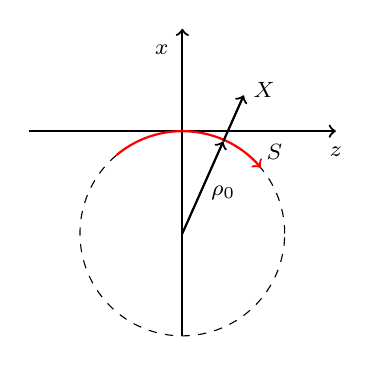
\begin{tikzpicture}[scale=1.3]
  \footnotesize
  % helper grid: comment for final drawing
  % \draw[help lines,step=.2] (0,0) grid (16.0,9.0);
  % \draw[help lines,line width=.6pt,step=1] (0,0) grid (16.0,9.0);
  % \foreach \x in {0,1,2,3,4,5,6,7,8,9,10,11,12,13,14,15,16}
  %      \node[anchor=north] at (\x,-0.1) {\x};
  % \foreach \y in {0,1,2,3,4,5,6,7,8,9}
  %     \node[anchor=east] at (-0.2,\y) {\y};

  % % text
  % \node [draw,rotate=90]  at (3.50,5.50)  {Injection};
  % % straight line and parabola
  % \draw [red,thick]          (0,0) -- (4,3);
  % \draw [black,thick,dashed] (0,0) parabola (4,4);
  % % bezier lines
  % \draw (6,0) .. controls (6,4) and (10,0) .. (10,4);
  % % circular shapes
  % \draw (5,5) circle (2cm);
  % \draw (7,2) ellipse (3cm and 1cm);
  % \draw (3,5) arc (0:75:3cm);
  % % filled rectangle



  % lower blms
%  \filldraw[fill=orange, draw=black] (9.2,3.8) rectangle (9.6,4.0);



  % % axes
  \draw[->,thick] (2,3) -- (5,3);
  \draw[->,thick] (3.5,1) -- (3.5,4);
  \draw[dashed] (3.5,2.0) circle (1.0);
  \draw[red,thick,->] (3.5,3.0) arc (90:40:1.0);
  \draw[red,thick,-] (3.5,3.0) arc (90:130:1.0);

  \draw[->,thick] (3.5,2) -- (3.9,2.9);
  \draw[->,thick] (3.9,2.9) -- (4.1,3.35);

  \node  at (3.9,2.4)  {$\rho_0$};
  \node  at (4.4,2.8)  {$S$};
  \node  at (5.0,2.8)  {$z$};
  \node  at (3.3,3.8)  {$x$};
  \node  at (4.3,3.4)  {$X$};

  % \draw[thick,->] (0,0) -- (0,4.5);

\end{tikzpicture}
  \caption{Transformation of the straight coordinate system $(x,y,z)$ into the curvilinear system $(X,Y,S)$. Based on \cite{wolski2014beam}.}
  \label{pic:15041799}
  \end{figure}
%
%
%
%
The full derivation is shown in Appendix \ref{hcurv} and is discussed in detail in \cite{wolski2014beam}. Assuming a horizontal bending, the position coordinates in the old and new coordinate system are related as follows
%
\begin{align}
  x &= (\rho_0 + X) \, \cos \left( h_x \, S \right) - \rho_0 \, , \notag \\
  y &= Y , \\
  z &= (\rho_0 + X) \, \sin \left( h_x \, S \right)  \notag \, ,
\end{align}
with the well-known curvature $h_x = \frac{1}{\rho_0}$ of the reference frame. From the generating function in \eqref{genF:rot}, the transformation of the momentum coordinates can be shown to be
\begin{align}
P_X &= p_x \,  \cos \left( h_x \, S \right) + p_z  \sin \left( h_x \, S \right) \, , \notag \\
P_Y &= p_y \, , \\
P_S &= p_z \, \left( 1 + h_x \, X \right)  \cos \left( h_x \, S \right) - p_x \, \left( 1 + h_x \, X \right)  \sin \left( h_x \, S \right) \, . \notag
\end{align}
%
Finally, the transformed vector potentials are given as 
%
\begin{align}
  A_X &= A_x \, \cos \left( h_x \, S \right) - A_z \, \sin \left( h_x \, S \right) \, , \notag \\
  A_Y &= A_y \, , \\ 
  A_S &= A_z \, \cos \left( h_x \, S \right) + A_x \, \sin \left( h_x \, S \right) \, . \notag 
\end{align}
%
Again, for convenience, a redefinition of the symbols used for the position coordinates is applied to have consistency in the tracking maps defined below $(X,Y,S) \rightarrow (x,y,s)$. The physical meaning of these quantities should be kept in mind when tracking maps are derived in curved coordinate systems.
%
The final Hamiltonian after this transformation is given by~\cite{Fjellstrom:1642385}
%
\begin{align}
  H = p_\sigma - (1+h_x(s)\,x) \, \left(  \sqrt{ (1+\delta)^2  - (p_x - \chi a_x(s))^2 - (p_y-\chi a_y(s))^2} + \chi a_s(s)  \right)\,. \label{eq:rawHamiltonian}
\end{align}
%
% The longitudinal magnetic vector potential with respect to $s$ is defined by the following relation
% %
% \begin{align}
% p_s = \frac{m_0 \, \gamma \, \dot{s}}{P_0} \, (1+h_xx)^2 + q (1+h_xx) \, \chi \, a_s \, .
% \end{align}
%
For the case of a straight coordinate system with $h_x=0$, the quantities described in the curved reference frame converge into those derived for the straight coordinate system. 

In the mono-isotopic limit of $m \rightarrow m_0$ and $q \rightarrow q_0$, which implies \mbox{$\chi \rightarrow 1$}, all derived equations converge to the standard expressions derived from the mono-isotopic Hamiltonian~\cite{CERN-SL-95-12}.
%
\subsubsection{Expansion}
%
%
The Hamiltonian presented in ~\eqref{eq:rawHamiltonian} is exact, thus without the usage of approximations. Depending on the complexity of the electromagnetic field of the beam-line element and the corresponding boundary conditions it can be useful to expand the square root in $\frac{(p_x-\chi a_x)^2 + (p_y - \chi a_y)^2}{(1+\delta)^2}$. By virtue of the normalization applied in \eqref{eq:normalization_H}, this is a small quantity, such that the second order Taylor expansion delivers a good approximation of the physical problem:
\begin{align}
H \approx p_\sigma - (1+h_x(s)x) \left[ (1+\delta) \left( 1 - \frac{1}{2} \frac{(p_x - \chi a_x(s))^2 + (p_y - \chi a_y(s))^2 }{(1+\delta)^2} \right) + \chi a_s(s) \right] \, . \label{eq:expanded_hamiltonian}
\end{align}  
The accuracy of tracking maps derived from the expanded Hamiltonian is studied for the example of a drift space in the mono-isotopic case in \cite{Fjellstrom:1642385}. It shows that the tracking maps derived from the exact and expanded Hamiltonian are in very good agreement if $p_x$ and $p_y$ are small. Significant differences arise only for values of $p_x$ and $p_y$ which are so large that the particle would be lost in the magnet aperture after only a few mm.

%
%
\section{Tracking Maps for Beam-Line Elements}\label{chap:trackingmaps}
%
In this section, the tracking maps for various types of individual beam line elements (such as drift space, dipole, quadrupole and RF cavity) are derived, based on the Hamiltonian for multi-isotopic particle beams introduced before. They are the baseline for the implementation of hiSixTrack, which was the main aim of this thesis project. 

For the dipole and the quadrupole, also the thick lens tracking maps are presented, although the implementation in hiSixTrack performs thin lens tracking. All implemented tracking maps, except for the drift space, are derived from the expanded multi-isotopic accelerator Hamiltonian in thin lens approximation. 

The symplecticity of the tracking maps for the different beam line elements is demonstrated by means of the Jacobian matrix in Appendix \ref{chap:sympl}. The technical implementation in hiSixTrack is presented in Appendix \ref{chap:implement}. 
%
%
\subsection{Drift Space}
% A drift space is a field-free region, in which the particles move on a straight line. If a particle enters a drift space region of length $L$ with the initial coordinates $x_i,x_i'$, the final angle and position $x_f,x_f'$ are given by the trivial relation
% \begin{align}
% \begin{pmatrix} x_f \\ x_f' \end{pmatrix} = \begin{pmatrix} 1 & L \\ 0 & 1 \end{pmatrix} \begin{pmatrix} x_i \\ x_i' \end{pmatrix} \, .
% \end{align}
% The full set of symplectic tracking maps is obtained by means of the Hamiltonian. 


\subsubsection{Exact Hamiltonian}
A drift space is defined by the absence of electromagnetic fields, thus the vector potential is zero in all directions. With regard to \eqref{eq:rawHamiltonian}, the Hamiltonian is then given by
\begin{align}
H = p_\sigma - \sqrt{(1+\delta)^2 - p_x^2 -p_y^2}  \, . \label{eq:full_H_drift}
\end{align}
Taking into account that $\delta$ is a function of $p_\sigma$ with the derivative $\PD{\delta}{p_\sigma}= \frac{\beta_0}{\beta}$, the equations of motion derived from this Hamiltonian are
\begin{alignat}{4}
x' &= \TD{x}{s} = \PD{H}{p_x} = \frac{p_x}{ \sqrt{(1+\delta)^2 - p_x^2 -p_y^2} } \, ,\quad \quad \quad \quad &p_x' &&= -\PD{H}{x} = 0 \, , \\
y' &= \TD{y}{s} = \PD{H}{p_y} = \frac{p_y}{\sqrt{(1+\delta)^2 - p_x^2 -p_y^2}}\, ,  \quad \quad &p_y' &&= -\PD{H}{y} = 0 \, , \\
\sigma' &=  \TD{\sigma}{s} = \PD{H}{p_\sigma} = \left( 1 - \frac{\beta_0}{\beta_z}  \right) \, ,    &p_\sigma' &&= -\PD{H}{\sigma} = 0 \, , 
\end{alignat}
where $\beta_z$ is defined as 
\begin{align}
\beta_z = \beta \, \frac{\sqrt{(1+\delta)^2 - p_x^2 -p_y^2}}{1+\delta}\,.
\end{align}
%
Starting from the equations of motion, the transformation of the initial set of coordinates $(\mathbf{q}^I,\mathbf{p}^I)$ at the beginning of the drift space is related to their final coordinates $(\mathbf{q}^F,\mathbf{p}^F)$ by the following set of equations
%
\begin{alignat}{4}
x^F & = x^I + \frac{p_x^I}{ \sqrt{(1+\delta)^2 - p_x^2 -p_y^2} } \,  L \, , \quad \quad \quad \quad \quad \quad &p_x^F &= p_x^I \, , \\
y^F & = y^I + \frac{p_y^I}{ \sqrt{(1+\delta)^2 - p_x^2 -p_y^2} } \,  L \, ,\quad \quad &p_y^F &= p_y^I \, , \\
\sigma^F & = \sigma^I + \left(1 - \frac{\beta_0}{\beta_z}\right) \,  L\, , \quad \quad &p_\sigma^F &= p_\sigma^I \, ,
\end{alignat}
%
where, $L$ denotes the length of the drift space. This type of mapping is referred to as a tracking map. 
\subsubsection{Expanded Hamiltonian}
Combining \eqref{eq:expanded_hamiltonian} and \eqref{eq:full_H_drift} results into the expanded Hamiltonian
\begin{align}
H \approx p_\sigma - \delta + \frac{1}{2} \, \frac{p_x^2+p_y^2}{(1+\delta)} \, . \label{eq:exp_drift}
\end{align}
Hamilton's equations of motion are then
\begin{alignat}{4}
x' &= \TD{x}{s} = \PD{H}{p_x} = \frac{p_x}{ (1+\delta) } \, , &p_x' &&= -\PD{H}{x} = 0 \, , \\
y' &= \TD{y}{s} = \PD{H}{p_y} = \frac{p_y}{ (1+\delta) }\, , \quad \quad &p_y' &&= -\PD{H}{y} = 0 \, , \\
\sigma' &=  \TD{\sigma}{s} = \PD{H}{p_\sigma} =  1 - \frac{\beta_0}{\beta} \left( 1 + \frac{1}{2} \, \frac{p_x^2 + p_y^2}{(1+\delta)^2}  \right)\, ,   \quad \quad \quad  &p_\sigma' &&= -\PD{H}{\sigma} = 0 \, .
\end{alignat}
Note the different definition of $x'$ with respect to the exact Hamiltonian. The resulting tracking map for the drift space from the expanded Hamiltonian yields
%
\begin{alignat}{4}
x^F &= x^I +   \frac{p_x^I}{1+\delta} \, L \, , &p_x^F &&= p_x^I \, , \\
y^F &= y^I +   \frac{p_y^I}{1+\delta} \, L \, , &p_y^F &&= p_y^I \, , \\
\sigma^F &=  \sigma^I - L \, \frac{\beta_0}{\beta} \left( 1 + \frac{1}{2} \, \frac{(p_x^I)^2 + (p_y^I)^2}{(1+\delta)^2}  \right) \, ,  \quad \quad \quad  &p_\sigma^F &&=  p_\sigma^I \, .
\end{alignat}
%
The direct comparison of $x'$ for the expanded and the exact drift space shows that they agree if $p_x$ and $p_y$ are small quantities. Since 2013, the exact Hamiltonian is implemented in SixTrack.

The modification of tracking maps for the drift space is not necessary for hiSixTrack, because the key quantity $\beta_0/\beta$ is defined in SixTrack as follows
\begin{align}
\frac{\beta_0}{\beta} = \frac{E}{p \, c} \, \frac{p_0 \, c}{E} \, .
\end{align}
When the correct energy and momentum are assigned to the heavy ions, this expression is also valid in the multi-isotopic case.
%which is valid also for particles of different species than the reference particle.

\subsection{Dipole} \label{chap:dipoleH}
For simplicity, parts of the following derivations are only considered for a horizontal bending ($x$ direction), but they are also valid for vertical bending by permuting $x$ and $y$. The uniform magnetic field in a horizontal bending dipole can be described by the vector potential~\cite{wolski2014beam}
\begin{align}
A_x = 0 \, , \quad \quad \quad A_y =0 \, , \quad \quad \quad A_s = -B_y x \, \left( 1- \frac{h_x x}{2 (1+h_x x)} \right)\, . \label{eq:pot:dipole}
\end{align}
Ideally, the vertical magnetic field $B_y$ is matched to the reference momentum and charge such that the bending radius of the reference particle yields $\rho_0=h_x^{-1}$. In reality, the magnet strength may differ from the reference, such that the ideal particle is bent with the radius $\rho^i=k_0^{-1}$ and 
\begin{align}
B_y = \frac{P_0 k_0}{q_0} \,  .
\end{align}
Combining \eqref{eq:rawHamiltonian} and \eqref{eq:pot:dipole} delivers the following Hamiltonian
\begin{align}
H = p_\sigma - (1+h_x x)\, p_z + \chi \, k_0 \left( x + \frac{h_x x^2}{2} \right) \, ,
\end{align}
%
with
%
\begin{align}
  p_z = \sqrt{(1+\delta)^2 - p_x^2 -p_y ^2} \, .
\end{align}
%
Omitting non-linear and constant terms delivers for the expanded Hamiltonian 
\begin{align}
H \approx p_\sigma - \delta - (h_x x) (1+\delta) + \frac{1}{2} \frac{p_x^2 + p_y^2}{(1+\delta)} + \chi \, k_0 \, \left(x + \frac{h_x x^2}{2}\right) \, . \label{eq:exp_dipole}
\end{align}
%
%
\subsubsection{Thick Dipole}
%
The following derivation is done assuming a sector magnet or a dipole with straight edges. With the expanded Hamiltonian and considering that $\delta$ is a function of $p_\sigma$ with the derivative $\frac{\mathrm{d} \delta}{\mathrm{d} p_\sigma} = \frac{\beta_0}{\beta}$, the equations of motion become
%
% CHECKED FOR ACCURACY 28.06.16 
% MATHEMATICA NOTEBOOK: DIPOLE_new
%
\begin{alignat}{4}
  x' &=  \PD{H}{p_x} = \frac{p_x}{1+\delta} \,, \quad \quad \quad \quad &p_x' &= -\PD{H}{x} = h_x \, (1+\delta) - \chi \, k_0 \, (1+h_x x)  \, , \label{eq:dipoleequationofmotion}  \\ 
  y' &= \PD{H}{p_y} = \frac{p_y}{1+\delta} \,, \quad \quad &p_y' &= -\PD{H}{y} = 0 ,   \label{eq:dipoleequationofmotiony}\\
  \sigma' &=  \PD{H}{p_\sigma} =  1 - \frac{\beta_0}{\beta} \left( 1+h_x x + \frac{1}{2} \frac{p_x^2 + p_y^2}{(1+\delta)^2} \right) \,, \quad \quad  &p_\sigma' &= -\PD{H}{\sigma} = 0 \, ,   \label{eq:dipoleequationofmotionz}
\end{alignat}
%
where $q_i' = \frac{\mathrm{d} q_i}{\mathrm{d} s}$. In the vertical direction, the dipole acts like a drift space. 

Starting from \eqref{eq:dipoleequationofmotion}, the horizontal motion can be described by the differential equation
\begin{align}
x''(s) + \frac{\chi \, h_x \, k_0}{(1+\delta)} \, x = \frac{h_x \, \delta}{(1+\delta)} + \frac{h_x - \chi \, k_0}{(1+\delta)} \, . \label{eq:diffeqdipole}
\end{align}
%
The homogeneous part of the equation describes an oscillation with frequency $\omega_x=\sqrt{\frac{\chi \, h_x \, k_0}{1+\delta}}$. Note that the inhomogeneous part of the differential equation \eqref{eq:diffeqdipole} represents the dispersion in the magnet. Compared to the corresponding mono-isotopic equation presented in \cite{DESY-95-189}, an additional term $\frac{h_x - \chi \, k_0}{(1+\delta)}$ appears, which takes into account the isotopic dispersion and a mismatched magnetic field. If the magnetic field is perfectly matched for the reference momentum ($h_x=k_0$), this term vanishes for particles of the reference species. 
%
%

The differential equation \eqref{eq:diffeqdipole} can be solved by a superposition of sine and cosine functions. The quantities $x^F$ and $y^F$ can be subsequently used to derive $p_x^F$ \mbox{and $p_y^F$} by integrating \eqref{eq:dipoleequationofmotion} and \eqref{eq:dipoleequationofmotiony}.  For convenience, the following quantities are introduced
\begin{alignat}{4}
S_x &= \sin \omega_x L \,, \quad \quad \quad &C_x &=  \cos \omega_x L \,, \label{eq:sx} \\ \omega_x^2 &= \frac{\chi \, h_x \, k_0}{1+\delta} \,,   &\Omega_x &= \frac{1+\delta}{k_0 \,\chi} - \frac{1}{h_x} \, . \label{eq:omx}
\end{alignat}
The resulting tracking map for the transverse coordinates is then given by
\begin{align}
% 
% x is correct 28.06.16
% SYMPLECTICITY FOR 4D CASE CHECKED
%
x^F &= x^I \, C_x + p_x^I \, \omega_x^{-1} \frac{S_x}{(1+\delta)} + \Omega_x \, \left(1 - C_x \right) \, , \label{eq:solution_thick_dipole}\\
%
%
p_x^F &= -x^I \, \omega_x \, (1+\delta) \, S_x + p_x^I \, C_x + (1+\delta) \, \Omega_x \, \omega_x \, S_x \, , \\
%
%p_x &\rightarrow - x \, \omega_x \, \tilde{S}_x + p_x \, C_x + \omega_x \,   \Omega_x \, \tilde{S}_x \, , \\ 
y^F &=  y^I + (y')^I \, L , \\
p_y^F &= p_y^I \, . \label{eq:tckdp4} %\\ 
%
% \sigma^F &= \sigma^I + L \, \left[ 1 - \frac{\beta_0}{\beta} - \frac{\beta_0}{\beta} \, \frac{1}{2} \, \left(\frac{p^I_y}{1+\delta} \right)^2 \right]  - \\ 
%  & \phantom{ \sigma^I +aaa} \frac{\beta_0}{\beta} \, \left[ \frac{S_x}{\omega_x} \, \left(x^I - \Omega_x \right) + \frac{p_x^I \, (1-C_x)}{(1+\delta) \, \omega_x^2} + L \, \Omega_x  \right] - \\
%  & \phantom{ \sigma^I + aaa} \frac{1}{8} \, \frac{\beta_0}{\beta} \, \frac{1}{(1+\delta)^2} \, \Bigg[ - 2 \, p_x^I \, (1+\delta) \, (x^I - \Omega_x) + \\  
%  & \phantom{ \sigma^I + aaaaaaaaaaaaaaaaaa} 2 \, L \, \left( \left(p_x^I\right)^2 +(1+\delta)^2\,\omega_x^2\,\left(x^I-\Omega_x\right)^2 \right) +  \\ 
%  & \phantom{ \sigma^I + aaaaaaaaaaaaaaaaaa} 2 \, p_x^I \, (1+\delta) \, \left(x^I-\Omega_x\right)\, \cos \left(2 \, \omega_x \, L \right) + \notag \\
%  & \phantom{ \sigma^I + aaaaaaaaaaaaaaaaaa} \frac{\sin \left(2 \, \omega_x \, L \right)}{\omega_x} \, \left( \left(p_x^I\right)^2 - (1+\delta)^2 \, \omega^2 \, \left(x^I - \Omega_x\right) \right) \Bigg]  \\
%
% \sigma &\rightarrow \sigma + L\left(1 - \frac{\beta_0}{\beta}\right) \\
%   & \qquad\, -\frac{\beta_0}{\beta} \Bigg[ \frac{h_x S_x}{\sqrt{G_x}} \cdot x + \frac{1-C_x}{h_x} \cdot p_x
%   + \frac{h_y S_y}{\sqrt{G_y}} \cdot y + \frac{1-C_y}{h_y} \cdot p_y
%   + \delta \left(2L - \frac{S_x}{\sqrt{G_x}} - \frac{S_y}{\sqrt{G_y}} \right) \Bigg] \\
%   & \qquad\, - \frac{1}{4}\frac{\beta_0}{\beta} \Bigg[ G_x \left(L-\frac{C_xS_x}{\sqrt{G_x}} \right)
%   \left(x - \frac{\delta}{h_x}\right)^2
%   + \left(L+\frac{C_xS_x}{\sqrt{G_x}} \right) \frac{p_x^2}{(1+\delta)^2}
%   -\left(x-\frac{\delta}{h_x}\right) \frac{2S_x^2}{1+\delta} \cdot p_x \\
%   & \qquad\, + G_y \left(L-\frac{C_yS_y}{\sqrt{G_y}} \right)
%   \left(y - \frac{\delta}{h_y}\right)^2 + \left(L+\frac{C_yS_y}{\sqrt{G_y}}\right) 
%   \frac{p_y^2}{(1+\delta)^2}
%   -\left(y-\frac{\delta}{h_y}\right)\frac{2S_y^2}{1+\delta} \cdot p_y \Bigg] \\
%
\end{align} 

The longitudinal coordinates can be derived by integrating \eqref{eq:dipoleequationofmotionz} after replacing $x,y,p_x$ \mbox{and $p_y$} by the transformed quantities. The resulting expression is identical to that derived for the mono-isotopic case in \cite{SixTrackLibManual}, with re-defined quantities in \eqref{eq:sx} and \eqref{eq:omx}.


\subsubsection{Thin Dipole}
Thick lens tracking is very demanding in terms of time and computing power. Also, the exact motion of the particle inside the magnet is often not required and the global tracking through a large accelerator like the LHC can be well approximated by thin lenses. The tracking routine used in hiSixTrack and in SixTrack for collimation studies is based on thin lens tracking, so the derivation of thin lens tracking maps is of particular interest. 

\newpage
The Hamiltonian in \eqref{eq:exp_dipole} can be decomposed into the expanded Hamiltonian $H_D$ of a drift space, defined in \eqref{eq:exp_drift}, and the contribution from electromagnetic fields $H_L$ as follows
%
\begin{align}
  H = H_D - h_x \, x \, (1+\delta) + \chi \, k_0 \, \left(x + \frac{h_x \, x^2}{2} \right) = H_D + H_L \, .
\end{align}
%
In the thin lens approximation, this Hamiltonian is changed to~\cite{DESY-95-189}
%
\begin{align}
 H = H_D + \bar{\delta}(s-s_0) \, L \, H_L \, , \label{eq:thin_H}
\end{align}
%
where $\bar{\delta}(s-s_0)$ is the Dirac $\delta$ distribution which is non-zero only at the center $s_0$ of the magnet~\cite{dirac:1958}. 
%
Starting from this Hamiltonian, the equations of motion are given by
\begin{align}
  x'    &= \frac{p_x}{(1+\delta)} \, , \label{eq:motion_thin_dipole}\\
  p_x'  &= L \, \bar{\delta}(s-s_0) \, \left[ h_x (1+\delta) - \chi \, k_0 \, (1+h_x \, x)  \right] \, ,\\
  y'    &= \frac{p_y}{(1+\delta)} \, ,\\
  p_y'  &= 0 \, , \\
  \sigma' &= 1 - \frac{\beta_0}{\beta} - \frac{\beta_0}{\beta} \, \left[ \frac{1}{2} \left(x'^2 + y'^2\right) \right] - \frac{\beta_0}{\beta} \, h_x \, x \, (1+\delta) \, \bar{\delta}(s-s_0) \, L \, , \\
  p_\sigma ' &= 0 \, .
\end{align}
%
The solution of the differential equations in the thin lens approximation are obtained by integrating over $s$, in the range from $s-\epsilon$ to $s+\epsilon$ in the limit of $\epsilon \rightarrow 0$. The tracking map for $x$ with the equation of motion given in \eqref{eq:motion_thin_dipole} is obtained as follows
%
\begin{align}
  x^F - x^I = \lim_{\epsilon \rightarrow 0} \left[ \int_{s_0 - \epsilon}^{s_0+\epsilon} \frac{p_x}{(1+\delta)} \, \mathrm{d}s \right] = 0 \, .
\end{align}
%
%
%
\input{pictures/16070702.tex}
  % #PHTHESIS FILE ORIGIN
  %/home/phermes/Dropbox/PhD/pictures/150922_weak_focusing/tikz/drawing.tex
%
%

Applying the same approach for the remaining quantities, the transformation rules for the dipole in thin lens approximation are given by
\begin{alignat}{4}
x^F &= x^I \, ,   &  p_x^F &= p_x^I + L \left[ h_x \, (1+\delta) - k_0 \, \chi \, (1 + h_x \, x^I)  \right]\, \label{eq:thindipolekick} , \\  
y^F &= y^I \, ,  &  p_y^F &= p_y^I\, ,\\ 
\sigma^F &= \sigma^I - \frac{\beta_0}{\beta} \, h_x \, x^I \, L \, , \quad \quad   & p_\sigma^F & = p_\sigma^I \, \label{eq:thindip02} .
\end{alignat}
%
% \begin{alignat}{4}
% x^F &= x^I \, , \label{eq:thindip01} \\ 
% p_x^F &= p_x^I + L \left[ h_x \, (1+\delta) - k_0 \, \chi \, (1 + h_x \, x^I)  \right]\, \label{eq:thindipolekick} ,\\ 
% y^F &= y^I \, ,  \\ 
% % \end{alignat}
% %
% % \begin{alignat}{4}
% p_y^F &= p_y^I\, ,\\ 
% \sigma^F &= \sigma^I - \frac{\beta_0}{\beta} \, h_x \, x^I \, L \, , \\
% p_\sigma^F & = p_\sigma^I \, \label{eq:thindip02} .
% \end{alignat}
%
The change in $p_x$ hence depends on the initial horizontal offset $x^I$. 

Two particles with the same set of $\chi$ and $\delta$ hence receive a different change in transverse momentum if they pass the dipole at two different initial offsets $x^I_1$ and $x^I_2$. The difference in the transverse momentum transfer is such that both particles are ultimately focused to a defined focal point, as illustrated in \figref{pic:15092201}. This effect is known as weak focusing~\cite{wolski2014beam}. 

%
The effect of dispersion is taken into account by the dependence on $\delta$ and $\chi$. The dispersive offset from chromatic offsets (chromatic dispersion) is which is a pure function of the particle velocity and hence $\delta$. The dispersive offset from the different mass to charge ratio (isotopic dispersion) is described by $\chi$. Chromatic and isotopic dispersion can compensate or enhance each other. 

For $x=0$, the change in $x'$ is given as 
\begin{align}
  (x')^F = (x')^I + h_x \, L - \frac{\chi}{1+\delta} \, k_0 \, L \, .
\end{align}
This shows that, in addition to the nominal bending $h_x \, L$, the particle receives a change of $x'$ that is proportional to $\frac{\chi}{1+\delta}$, well known from \eqref{eq:15080401}. This shows that the generic Hamiltonian delivers the expected dynamics and correctly accounts for the isotopic dispersion.

%In the mono-isotopic case $\chi \rightarrow 1$ and with perfectly matched magnetic field $k_0=h_x$, the \eqref{eq:thindipolekick} yields the well known shape (see \cite{CERN-SL-95-12})
%\begin{align}
%p_x^F = p_x^I + \delta h_x L - h_x^2 \, L \, x^I \, .
%\end{align} 




  % \begin{figure}[t]
  % \centering
  % \includegraphics[width=0.4\textwidth]{pictures/15092201.pdf}
  % \caption{Bending behaviour in a magnetic dipole field for two particles starting with different initial conditions.}  
  % \label{pic:15092201}
  % %/home/phermes/Dropbox/PhD/pictures/150922_weak_focusing/drawing-compiled.pdf
  % \end{figure}

\subsection{Thin Transverse Kicker Magnet}

  \begin{figure}[t]
  \centering
  \includegraphics[width=0.7\textwidth]{pictures/15112403.pdf}
  \caption{Schematics of a transverse kicker magnet. Kicker magnets are dipole magnets where the reference trajectory is not bent, thus $h_x=0$. }  
  \label{pic:15112403}
  %/home/phermes/Dropbox/PhD/pictures/151125_kickermagnet/tikz_drawing-crop.pdf
  \end{figure}


Transverse kicker magnets are used in accelerators as the LHC to control the beam orbit. Technically they are identical to bending magnets, with the exception that $h_x=0$, so the reference trajectory in these magnets is not bent. The Hamiltonian for a transverse kicker magnet in thin lens approximation is given by
%
\begin{align}
  H=  H_D + \chi \, k_0 \, L \, \bar{\delta}(s-s_0) \, .
\end{align}
%
The resulting equations of motion lead to the following transport map
\begin{alignat}{4}
p_x^F & = p_x^I - k_0 \, \chi \, L\, \label{eq:kickermagnet} ,\\ 
p_y^F & = p_y^I\, ,\\ 
p_\sigma^F & = p_\sigma^I \, .
\end{alignat}

Taking into account that $x' = \frac{p_x}{(1+\delta)}$, the transformation of $x'$ yields
%
\begin{align}
  (x')^F = (x')^I - k_0 \, L \, \frac{\chi}{(1+\delta)} \, .
\end{align}
As expected from \eqref{eq:15080401}, the change in $x'$ is proportional to $\frac{\chi}{1+\delta}$.

\subsection{Quadrupole}
%
The vector potential of a horizontal or vertical quadrupole magnet is given by~\cite{CERN-SL-95-12}
\begin{align}
A_x = 0 \, , \quad \quad \quad A_y = 0 \,, \quad \quad \quad A_z = - \frac{1}{2} \, g \, (y^2 -x^2) \, .
\end{align}
%
Expressed in the normalized coordinates, the longitudinal vector potential becomes
%
\begin{align}
a_z = - \frac{1}{2} \frac{q_0}{P_0} g  \, (y^2 -x^2)  = - \frac{1}{2} \, k \,  (y^2 -x^2) \, .
\end{align}
The quantity $g$ is the quadrupole gradient introduced in \chapref{quad:intro}, and $k=\frac{q_0}{P_0} g$ is the normalized quadrupole gradient which has the unit $[k] = \text{m}^{-2}$. The optics of a machine in a certain configuration is defined by a full set of $k_i$ with $i= 1,...,N_q$, where $N_q$ is the number of quadrupoles in the machine. Thanks to the definition of the normalized quadrupole gradient (see \eqref{norm:quadstr}), the machine optics can be described by identical values valid for different energies, even if in reality the magnet currents are ramped with increasing beam energy. 

The reference trajectory passes through the center of the quadrupole, where no magnetic field is present and is hence straight with $h_x=0$. The exact Hamiltonian of a quadrupole yields 
\begin{align}
H = p_\sigma - \sqrt{(1+\delta)^2 - p_x^2 -p_y^2} + \frac{1}{2} \, k \, \chi\, (x^2 -y^2) \, .
\end{align}

\subsubsection{Thick quadrupole}
%
%
The expanded Hamiltonian for the quadrupole is then given by
\begin{align}
H = p_\sigma + \frac{1}{2} \frac{p_x^2+p_y^2}{(1+\delta)} + \frac{1}{2} \, \chi \, k  \, (x^2 -y^2) -\delta \, . \label{eq:quad_exp_H}
\end{align}
Hamilton's equations deliver the following equations of motion
%
\begin{alignat}{4}
x'      &= \PD{H}{p_x} = \frac{p_x}{(1+\delta)} \,,\quad \quad \quad &p_x' &= - \PD{H}{x} = - \chi\, k\, x \, ,  \\
y'      &= \PD{H}{p_y} = \frac{p_y}{(1+\delta)} \,,\quad \quad \quad &p_y' &= - \PD{H}{y} = \phantom{-} \chi\,  k \,  y \, , \\
\sigma' &= \PD{H}{p_\sigma} = 1- \frac{\beta_0}{\beta} \, \left[ 1 + \frac{1}{2} \frac{p_x^2 + p_y^2}{(1+\delta)^2}  \right] \,, \quad \quad \quad &p_\sigma' &= - \PD{H}{\sigma} =  \phantom{-}  0 \, .
\end{alignat}
To facilitate the solution of the equations of motion, the quantity $\omega$ is defined as
\begin{align}
 \omega^2 = \frac{|\chi \,  k|}{(1+\delta)} \, .
\end{align}
Using these relations, the transverse motion can be described by two differential equations of the same type
\begin{align}
x'' + \omega^2 x &= 0 \, , \label{eq:quadeq1} \\
y'' - \omega^2 y &= 0 \, .
\end{align}
%
The transverse transport map is the general solution of the two differential equations 
\begin{alignat}{8}
x^F &= C_x x^I &&+ S_x \frac{p_x^I}{(1+\delta)} \, ,\quad \quad \quad \quad &p_x^F &= C_x p_x^I &&-  S_x \, \omega^2 x^I \, (1+\delta) \, , \\ 
y^F &= C_y y^I &&+ S_y \frac{p_y^I}{(1+\delta)} \, , &p_y^F &= C_y p_y^I &&+  S_y \, \omega^2 y^I  \, (1+\delta) \, .  %\\
% \sigma & \rightarrow \sigma && &p_\sigma &\rightarrow \sigma + &&\left( 1 - \frac{\beta_0}{\beta} \right) L  \, & \\
%  & && & & &&-\frac{\omega^2}{4} \frac{\beta_0}{\beta} \left( [S_x C_x -L] x^2 - [S_y C_y -L] y^2 \right) \notag \\
%   & && & & &&-\frac{\omega^2}{2} \frac{\beta_0}{\beta} \left( -S_x^2 \frac{x p_x}{1+\delta} +S_y^2 \frac{y p_y}{1+\delta} \right) \notag \\
%  & && & & &&-\frac{1}{4} \frac{\beta_0}{\beta} \left( [L+S_xC_x] \frac{p_x^2}{(1+\delta)^2} + [L+S_yC_y] \frac{p_y^2}{(1+\delta)^2} \right) . \notag
\end{alignat}
The quantities $C_u$ and $S_u$ are defined as follows
\begin{alignat}{4}
C_x = &\begin{cases}  \cos \left( \omega L \right)  & \text{if} \quad  \chi \, k>0 \\ 
\cosh \left( \omega L \right)  & \text{if} \quad  \chi \, k<0 \end{cases} \, , \quad \quad \quad&S_x = &\begin{cases}  \omega^{-1}  \sin \left( \omega L \right)  & \text{if} \quad  \chi \, k>0 \\ \omega^{-1}\sinh \left( \omega L \right)  & \text{if} \quad  \chi \, k<0 \end{cases} \label{eq:quad_solution1}
\, , \\ 
C_y = &\begin{cases}  \cosh \left( \omega L \right)  & \text{if} \quad  \chi \, k>0 \\ 
\cos \left( \omega L \right)  & \text{if} \quad  \chi \, k<0 \end{cases} \, ,\quad \quad \quad&S_y = &\begin{cases}  \omega^{-1}  \sinh \left( \omega L \right)  & \text{if} \quad  \chi \, k>0 \\ \omega^{-1}\sin \left( \omega L \right)   & \text{if} \quad  \chi \, k<0 \end{cases} \label{eq:quad_solution2}
\, . 
\end{alignat}

The longitudinal coordinates are identical to those derived in \cite{SixTrackLibManual}.


\subsubsection{Thin Quadrupole}

Following the Eqs.~(\ref{eq:thin_H}) and (\ref{eq:quad_exp_H}), the following Hamiltonian can be derived to describe the quadrupole in thin lens approximation
%
\begin{align}
  H = H_D + \frac{1}{2} \, \bar{\delta}(s-s_0) \, L \, \chi \, k \, (x^2-y^2) \, .
\end{align}
The corresponding transfer map for the kick by a thin-lens quadrupole yields
\begin{alignat}{8}
x^F &= x^I \, ,  \quad \quad \quad \quad &p_x^F &=  p_x^I &&-  \chi \, k \,  L \, x^I \, ,  \label{quad1}\\ 
y^F &= y^I \, ,  \quad \quad \quad \quad &p_y^F &=  p_y^I &&+  \chi \, k\,  L \, y^I \, , \label{quad2}\\
\sigma^F &= \sigma^I \, ,  \quad \quad \quad \quad &p_\sigma^F &=  p_\sigma^I \,. &&  &
\end{alignat}
This transfer map corresponds to a focusing lens  in horizontal and a defocusing lens in vertical direction (if $\chi \, k>0$ and vice versa for $\chi \, k <0$). The transformation of $x'$ and $y'$ is given as
\begin{align}
 (x')^F &= (x')^I - k \, L \, x^I \, \frac{\chi}{1+\delta} \, , \\
 (y')^F &= (y')^I + k \, L \, y^I \, \frac{\chi}{1+\delta} \, .
\end{align}
The focal length for the different isotopes is proportional to $\frac{\chi}{(1+\delta)}$, in line with the expectation.

\subsection{Thin Multipole} \label{chap:multipole}
Higher order magnetic fields are described in a more generic way by\footnote{In some references, e.g. in \cite{wiedemann1999particle}, the multipole field is defined as $B_y+i\,B_x = \sum_{n} \frac{(b_n+i \, a_n)}{n!} \, \left( \frac{x+i \, y}{r_0} \right)^{n-1}$. The multipole coefficients are defined differently than here, but the underlying physics remains unchanged.}~\cite{wolski2014beam}
%
\begin{align}
  B_y + i B_x = \sum_{n=1}^{\infty} (b_n + i a_n) \, \left( \frac{x+iy}{r_0} \right)^{n-1} \, . \label{eq:multiB}
\end{align}
%
In this context, $n$ is the multipole order, $b_n,a_n$ are the multipole coefficients which describe the field orientation for the contribution of each multipole order~\cite{wolski2014beam} and the quantity $r_0$ is a reference radius. The well-known dipole and quadrupole fields described in the previous sections correspond to the multipole orders $n_D=1$ and $n_Q=2$. In a perfect multipole of the order $n$, all remaining multipole coefficients yield zero.

The magnetic field described in \eqref{eq:multiB} corresponds to the following vector potential
%
\begin{align}
A_x = 0 \, , \quad \quad \quad A_y = 0 \, , \quad \quad \quad A_z = - \text{Re} \sum_{n=1}^{\infty} (b_n + i a_n) \frac{(x+i y)^n}{n \, r_0^{n-1}} \, .
\end{align} 
%
Inserting this vector potential the Hamiltonian in thin lens approximation yields
%
\begin{align}
  H = H_D - \frac{q_0}{P_0} \, \chi \, L \, \bar{\delta}(s-s_0) \, \text{Re} \, \left[ \sum_{n=1}^\infty (b_n + i \, a_n) \, \frac{(x+i \, y)^n}{n \, r_0^{n-1}}  \right]  \, .
\end{align}
%
The resulting tracking map for the thin multipole kick is
%
\begin{alignat}{8}
x^F & =  x^I \, ,  \quad \quad \quad \quad &p_x^F &=   p_x^I &&-  \chi \, L \, \text{Re} \left[ \sum_{n=1}^\infty (k_n+ i \, \hat{k}_n) \, (x+i\,y)^{n-1}    \right] \,, \\ 
y^F & =  y^I \, ,  \quad \quad \quad \quad &p_y^F &=  p_y^I && -  \chi \, L \, \text{Re} \left[ \sum_{n=1}^\infty \, i (k_n+ i \, \hat{k}_n) \, (x+i\,y)^{n-1}    \right] \,,\\ 
\sigma^F & =  \sigma^I \, ,  \quad \quad \quad \quad &p_\sigma^F &=  p_\sigma^I \,, &&  &
\end{alignat}
%
where $k_n$ and $\hat{k}_n$ are defined as
%
\begin{align}
  k_n = \frac{q_0}{P_0} \, \frac{a_n}{r_0^{n-1}} \quad \text{and} \quad   \hat{k}_n = \frac{q_0}{P_0} \, \frac{b_n}{r_0^{n-1}} \, .
\end{align}
These transformations are very demanding in terms of computing time. SixTrack therefore calculates multipole fields of higher order than quadrupoles using a Horner scheme (see \chapref{chap:implhst}).

\subsection{Accelerating RF Cavity}
  % \begin{figure}[t]
  % \centering
  % \includegraphics[width=0.8\textwidth]{pictures/15081101.jpg}
  % \caption{Principle of the beam acceleration by means of RF cavities. The structure generates a longitudinal electric field. The wavelength of this }  
  % \label{pic:15081101}
  % %/home/phermes/Documents/1435503941_77cff2f9fcf76f625a60aa3135ed2c87.jpg
  % \end{figure}


The energy gain $\Delta E$ a particle receives at the position $s$ inside an accelerating cavity operated in the  lowest order mode can be \mbox{approximated by}
%
\begin{align}
 \frac{\mathrm{d} \Delta E}{\mathrm{d} s} = q \,  V(s) \, \sin \left( 2 \pi \, \frac{h}{C} \, \sigma + \phi \right) \, , \label{eq:rfEkcik}
\end{align}
%
where $V(s)$ is the longitudinal electric field, $h$ is the harmonic number, $\phi$ is the phase and $C$ is the circumference of the accelerator. The dependence of $V$ on $s$ complicates the solution of the equations of motion and is therefore not explicitly considered in the magnetic vector potential. Rather, the electric field is averaged over the length of the cavity which is summarized in the mean electric field $U$~\cite{wolski2014beam}
%
\begin{align}
  U = \frac{1}{L} \, \int_{-L/2}^{L/2} V(s) \, \mathrm{d} s \, .
\end{align}
%
This approximation leads to the following vector potential for a cavity~\cite{CERN-SL-95-12}
%
\begin{align}
A_x = A_y =0 \, \quad \quad A_s = - \frac{1}{\beta_0 c} \,  \frac{C}{2 \pi \, h} \,  U \,  \cos \left( \frac{2 \pi \, h}{C} \, \sigma + \phi  \right) \, .
\end{align}
%
The resulting expanded Hamiltonian for a thin cavity is then given by
%
\begin{align}
  H = H_D + \chi \, q_0 \, \frac{1}{\beta_0^2}\, \frac{U}{E_0} \, \frac{C}{2 \pi \, h}   \, \cos \left( \frac{2 \pi \, h}{C} \, \sigma + \phi  \right) \, L \, \bar{\delta}(s-s_0) \, .
\end{align}

%
From this Hamiltonian, the transfer map can be deduced as
%
\begin{alignat}{8}
x^F & =  x^I \, ,  \quad \quad \quad \quad &p_x^F &=   p_x^I \, , && \\ 
y^F & =  y^I \, ,  \quad \quad \quad \quad &p_y^F &=  p_y^I \, ,&&  \\ 
\sigma^F & =  \sigma^I \, ,  \quad \quad \quad \quad &p_\sigma^F &=  p_\sigma^I + \chi \, q_0 \, \frac{1}{\beta_0^2}  \, \frac{U}{E_0} \, L \, \sin \left(  \frac{2 \pi \, h}{C} \, \sigma + \phi \right) \, .   &&  &
\end{alignat}
%
The change in $p_\sigma$ is, as expected, proportional to $q\, \frac{m_0}{m}$. Using the relation between $p_\sigma$ and $E$, the energy transfer from the accelerating RF cavity of length $L$ corresponds to the expression given in \eqref{eq:rfEkcik} and yields
%
\begin{align}
  \Delta E = q \, U \, L \, \sin \left(  \frac{2 \pi \, h}{C} + \phi \right) \, .
\end{align}
This transformation is implemented in hiSixTrack.


\newpage
\section{Multi-Isotope Tracking in hiSixTrack}

The new heavy-ion tracking tool hiSixTrack, which was developed for this thesis, is based on the multi-isotopic symplectic tracking maps derived in the previous chapter. In contrast to the STIER approach, hiSixTrack tracks the heavy ions with their correct physical properties instead of tracking protons with ion-equivalent rigidities. This generic approach required extensive changes of the physics implemented in SixTrack. 

\vspace{0.2cm}

In this section, the changes introduced in hiSixTrack are discussed qualitatively and individual features are benchmarked against other simulation tools. A more detailed technical overview, including examples of source code, is given in Appendix \ref{chap:impl:hist}. 



\subsection{Implementation of hiSixTrack} \label{chap:implhst}

With respect to SixTrack, the new tool hiSixTrack must provide additional arrays containing information about the particle mass, charge number and nucleon number to keep track of the ion species and apply the correct physics models. Also new arrays storing information about $\chi$ and auxiliary quantities derived from it are introduced. 
\vspace{0.2cm}

The definition of $\chi$ requires to load and store information about the reference species. To define the latter, a dedicated \texttt{HION} block is introduced in the \texttt{fort.3} file. In this block, the nuclear charge number, mass number and physical particle mass (in GeV/$c^2$) are given by the user. 
\vspace{0.2cm}

In the standard version of SixTrack, the quantity $\delta$ is defined as the relative momentum offset. In hiSixTrack, the definition is changed to obey the multi-isotopic definition given in \eqref{eq:15010701}:
%
\begin{align}
  \delta = \frac{P - P_0}{P_0}\quad \quad  \rightarrow \quad \quad \delta = \frac{P \frac{m_0}{m} - P_0}{P_0} \, .
\end{align}

With the new definition of $\delta$ and the information on $\chi$ available, the SixTrack tracking maps were modified following the thin lens tracking maps derived from the generalized Hamiltonian, presented in the previous chapter. Magnetic elements in SixTrack and hiSixTrack are implemented up to 20th order. However, for higher order fields than quadrupoles, the transformation is not calculated over the multipole equations presented in \chapref{chap:multipole}. Instead, the magnetic field acting on the particle is determined by several geometric transformations ultimately followed by the tracking map of a quadrupole (Horner Scheme)~\cite{SixTrackref01}.
\newpage
Instead of the transverse canonical momenta $p_x$ and $p_y$, SixTrack and hiSixTrack compute the evolution of $x',y'$. As an example, the tracking map for a thin-lens quadrupole is modified in hiSixTrack to obey \eqref{quad1} and \eqref{quad2}:
%
\begin{align}
  (x')^F = (x')^I + \frac{k \, L}{1+\delta} \, x^I \quad \quad \rightarrow \quad \quad   (x')^F = (x')^I + \frac{\chi \, k \, L}{1+\delta} \, x^I \, .
\end{align}

Further details on the implementation are given in Appendix \ref{chap:implement}. The new tracking routine for multi-isotopic heavy-ion tracking was extensively tested and benchmarked. The results of these tests are presented in the following sections.





\subsection{Benchmarking of Ion Tracking in hiSixTrack}

hiSixTrack provides symplectic tracking with multipole contributions to the same order as STIER. Hence, both simulation tools should simulate identical particle tracks when RF cavities and scattering in collimators are not included. In this section, the hiSixTrack tracking routine is benchmarked for all relevant scenarios against the tracking in STIER.  All simulation cases to study the accuracy of the implementation of hiSixTrack are listed in \tabref{tab:simucases}.

\begin{table}[b]
\centering
\caption{Simulation cases to benchmark hiSixTrack against STIER.}
\label{tab:simucases}

\begin{tabular}{rrl}
\toprule 
$\delta$ & $\chi$   & Description                                                                            \\ \midrule
0        & 1        & On-momentum tracking of particles of the reference species               \\
0        & $\neq 1$ & On-momentum tracking of isotopes different from the reference species  \\
$\neq 0$ & 1        & Off-momentum tracking of the reference ion species                                     \\
$\neq 0$ & $\neq 1$ & Off-momentum tracking of particles different from the reference species                   \\ \bottomrule
\end{tabular}
\end{table}


% %
% \begin{enumerate}
%     \item Study of the betatron motion for on-momentum particles of the reference species ($\delta = 0$; $\chi=1$),
%     \item Tracking of different isotopes with ideal momentum to study the modelling of the isotopic dispersion  ($\delta =0$, $\chi \neq 1$),
%     \item Tracking of off-momentum particles of the reference species to study the modelling of the chromatic dispersion ($\delta \neq 0$, $\chi =1$),
%     \item Tracking of off-momentum particles of an unmatched species ($\delta \neq 0$, $\chi \neq 1$).
% \end{enumerate}

All simulations assume the reference isotope to be \lead. Collimators and RF cavities are not included in the simulations.

\subsubsection{Betatron Motion without Dispersion}

% \begin{figure}[t]  
%     \centering
%     \includegraphics[width=0.9\textwidth]{pictures/16042801.pdf}
%     \includegraphics[width=0.9\textwidth]{pictures/16042801.pdf}
%     \caption{Horizontal particle tracks, simulated with hiSixTrack (top) and STIER (bottom), for on-momentum particles of the reference species. All particles start from IP1 on the surface of an horizontal annular halo at an amplitude of $5.7\,\sigma$.}  
%     \label{pic:16042801}    %/afs/cern.ch/work/p/phermes/private/150629_coupling_ions/hiSix/160316_runI_2011/runI.tracks/run_00001/betatron_benchmark.pdf
% \end{figure}



\begin{figure}[t]
  \centering
  \begin{tikzpicture}
    \node[anchor=south west,inner sep=0] (image) at (0,0) {\includegraphics[width=1.0\linewidth]{pictures/16091508.pdf}};
  \node [x={(image.south east)},y={(image.north west)}]                   at (0.90,0.87)    {hiSixTrack};
  \node [x={(image.south east)},y={(image.north west)}]                   at (0.90,0.45)    {STIER};

  % \node [draw,rotate=0 ,x={(image.south east)},y={(image.north west)}]                   at (0.22,0.96)    {text1};
  % \node [draw,rotate=0 ,x={(image.south east)},y={(image.north west)},anchor=west]       at (0.22,0.80)    {text2};
  % \draw[->,color=black,thick,x={(image.south east)},y={(image.north west)}]             (0.42,0.22) -- (0.37,0.23);

%  \draw[help lines,step=.05,x={(image.south east)},y={(image.north west)}] (0,0) grid (1,1);
%  \draw[help lines,line width=.6pt,step=0.1,x={(image.south east)},y={(image.north west)}] (0,0) grid (1,1);
%  \foreach \x in {0,0.1,0.2,0.3,0.4,0.5,0.6,0.7,0.8,0.9,1.0}
%       \node[anchor=north,x={(image.south east)},y={(image.north west)}] at (\x,-0.01) {\x};
%  \foreach \y in {0.0,0.1,0.2,0.3,0.4,0.5,0.6,0.7,0.8,0.9,1.0}
%      \node[anchor=east,x={(image.south east)},y={(image.north west)}] at (-0.01,\y) {\y};

  \end{tikzpicture}
  \caption{Horizontal particle tracks, simulated with hiSixTrack (top) and STIER (bottom), for on-momentum particles of the reference species. All particles start from IP1 on the surface of an horizontal annular halo at an amplitude of $5.7\,\sigma$.}  
  \label{pic:16042801}
  %/afs/cern.ch/work/p/phermes/private/150629_coupling_ions/hiSix/160316_runI_2011/runI.tracks/run_00001/betatron_benchmark.pdf
  \end{figure}






The betatron motion in hiSixTrack is benchmarked against STIER by comparing the tracks of on-momentum particles ($\delta = 0$) of the respective reference species ($\chi=1$) with identical starting conditions in IP1. The simulations with hiSixTrack and STIER are carried out for 100 particles starting with identical initial coordinates. The starting conditions are randomly sampled on the surface of a horizontal annular halo at 5.7$\,\sigma$, which corresponds to the half gap of the primary collimator in the 2011 heavy-ion run.  As an example, the betatron motion simulated with hiSixTrack and STIER for ten of these particles is shown in \figref{pic:16042801}. 
\newpage
The tracking is performed over $10^6$ turns through the magnetic lattice of the LHC for a particle energy of $3.5\,Z\,$TeV. The optical settings correspond to the configuration of the 2011 heavy-ion run with crossing and separation bumps switched on in all experimental IRs, except for IR1. 

The comparison shows that the tracks simulated with STIER and hiSixTrack are identical within the precision of the floating point numbers (15 significant digits) for all study cases.  This does not imply that particles can be tracked with such a precision. Rather, it demonstrates that the numeric reproducibiliy is maintained in hiSixTrack.

Additional tests in which the particles started at different betatron amplitudes delivered the same result.


\newpage

\subsubsection{Tracking of different Isotopes without chromatic Dispersion}




In this set of simulations, the modeling of isotopic dispersion in hiSixTrack is benchmarked against STIER. Particles of different isotopes are tracked without initial betatron amplitude or offset in momentum per mass. The optical lattice used for the simulation is matched to \lead and corresponds to the configuration of the 2011 heavy-ion run. Crossing and separation bumps are applied in all IRs, except IP1. 

Six different isotopes were chosen to be tracked, to cover a broad spectrum of $\chi$ values. They are listed in \tabref{tab:15080501}. The tracks simulated with hiSixTrack and STIER are illustrated in \figref{pic:15080501}. The particle tracks of all isotopes except for $^{207}$Pb$^{82+}$ and $^{207}$Tl$^{81+}$ were simulated for less than one turn through the LHC, because the dispersive offset becomes too large (SixTrack stops the particle tracking when amplitudes of 1\,m are reached). For the same reason, the isotope $^{207}$Pb$^{82+}$ can only be tracked over $100$ turns. For \iso{207}{Tl}{81+}, the tracking is performed over $10^6$ turns.

Also in this study case, the tracks simulated with both tools fully agree within the numeric precision. The tracking maps implemented in hiSixTrack hence deliver the same tracking behavior as the tracking with SixTrack with ion-equivalent rigidities. 



\begin{figure}[htbp]
  \centering
  \begin{tikzpicture}
    \footnotesize
    \node[anchor=south west,inner sep=0] (image) at (0,0) {\includegraphics[width=0.9\linewidth]{pictures/16091605.pdf}};
  \node [draw,fill=white,x={(image.south east)},y={(image.north west)}]                   at (0.60,0.89)    {hiSixTrack};
  \node [draw,fill=white,x={(image.south east)},y={(image.north west)}]                   at (0.60,0.46)    {STIER};
  % \node [draw,rotate=0 ,x={(image.south east)},y={(image.north west)}]                   at (0.22,0.96)    {text1};
  % \node [draw,rotate=0 ,x={(image.south east)},y={(image.north west)},anchor=west]       at (0.22,0.80)    {text2};
  % \draw[->,color=black,thick,x={(image.south east)},y={(image.north west)}]             (0.42,0.22) -- (0.37,0.23);

%  \draw[help lines,step=.05,x={(image.south east)},y={(image.north west)}] (0,0) grid (1,1);
%  \draw[help lines,line width=.6pt,step=0.1,x={(image.south east)},y={(image.north west)}] (0,0) grid (1,1);
%  \foreach \x in {0,0.1,0.2,0.3,0.4,0.5,0.6,0.7,0.8,0.9,1.0}
%       \node[anchor=north,x={(image.south east)},y={(image.north west)}] at (\x,-0.01) {\x};
%  \foreach \y in {0.0,0.1,0.2,0.3,0.4,0.5,0.6,0.7,0.8,0.9,1.0}
%      \node[anchor=east,x={(image.south east)},y={(image.north west)}] at (-0.01,\y) {\y};

  \end{tikzpicture}
  \caption{Heavy-ion tracks for different on-momentum ($\delta=0$) isotopes unmatched to the magnetic lattice ($\chi\neq1$) starting with the same initial conditions in IP1, simulated with hiSixTrack (top) and STIER (bottom).}  
  \label{pic:15080501}
  %/home/phermes/Dropbox/PhD/notebooks/graphics/isodisp.pdf
  \end{figure}




\begin{table}[htbp]
\centering
\caption{Isotopes used for the benchmarking of the heavy-ion tracking. Values for $\chi$ and $\delta_\text{eff}$ are computed with respect to the reference isotope \lead. The masses correspond to the fully stripped ions and are extracted from FLUKA. The rest mass of \lead is 193.688\,GeV/$c^2$.}
\label{tab:15080501}

\begin{tabular}{cccrcc}
\toprule
Element & $A$ & $Z$ & $m$ [GeV/$c^2$] & $\chi$   & $\delta_\text{eff}$ \\ \midrule
H       & \phantom{12}1   & \phantom{1}1   & 0.938         & 2.51744  & -0.6030              \\
H       & \phantom{12}3   & \phantom{1}1   & 2.809      & 0.84090  & \phantom{-}0.1892              \\
He      & \phantom{12}4   & \phantom{1}2   & 3.727         & 1.26740  & -0.2110              \\
Au      & 206 & 79  & 191.833      & 0.97273  & \phantom{-}0.0280             \\
Pb      & 207 & 82  & 192.755      & 1.00484  & -0.0048             \\
Tl      & 207 & 81  & 191.823      & 0.99741       & \phantom{-}0.0026           \\
Tl      & 208 & 81  & 193.693      & 0.98778 & \phantom{-}0.0124           \\ \bottomrule
\end{tabular}
\end{table}



\subsubsection{Tracking of the Reference Species with Momentum Offset}



\begin{figure}[b]
  \centering
  \begin{tikzpicture}
    \footnotesize
    \node[anchor=south west,inner sep=0] (image) at (0,0) {\includegraphics[width=0.85\linewidth]{pictures/16091608.pdf}};
  \node [draw,fill=white,x={(image.south east)},y={(image.north west)}]                   at (0.70,0.95)    {hiSixTrack};
  \node [draw,fill=white,x={(image.south east)},y={(image.north west)}]                   at (0.70,0.48)    {STIER};

  % \node [draw,rotate=0 ,x={(image.south east)},y={(image.north west)}]                   at (0.22,0.96)    {text1};
  % \node [draw,rotate=0 ,x={(image.south east)},y={(image.north west)},anchor=west]       at (0.22,0.80)    {text2};
  % \draw[->,color=black,thick,x={(image.south east)},y={(image.north west)}]             (0.42,0.22) -- (0.37,0.23);

%  \draw[help lines,step=.05,x={(image.south east)},y={(image.north west)}] (0,0) grid (1,1);
%  \draw[help lines,line width=.6pt,step=0.1,x={(image.south east)},y={(image.north west)}] (0,0) grid (1,1);
%  \foreach \x in {0,0.1,0.2,0.3,0.4,0.5,0.6,0.7,0.8,0.9,1.0}
%       \node[anchor=north,x={(image.south east)},y={(image.north west)}] at (\x,-0.01) {\x};
%  \foreach \y in {0.0,0.1,0.2,0.3,0.4,0.5,0.6,0.7,0.8,0.9,1.0}
%      \node[anchor=east,x={(image.south east)},y={(image.north west)}] at (-0.01,\y) {\y};

  \end{tikzpicture}
  \caption{Particle tracks of  ten \lead ions with different $\delta$, simulated with hiSixTrack (top) and STIER (bottom).}  
  \label{pic:16091101}
  %/afs/cern.ch/work/p/phermes/private/150629_coupling_ions/hiSix/160316_runI_2011/runI.tracks/run_00001/offenergy_ref.pdf
  \end{figure}



% \begin{figure}[htbp]
%   \centering
%   \begin{tikzpicture}
%     \node[anchor=south west,inner sep=0] (image) at (0,0) {\includegraphics[width=0.8\linewidth]{pictures/16091102.pdf}};
%   % \node [draw,rotate=90,x={(image.south east)},y={(image.north west)}]                   at (0.50,0.50)    {text0};
%   % \node [draw,rotate=0 ,x={(image.south east)},y={(image.north west)}]                   at (0.22,0.96)    {text1};
%   % \node [draw,rotate=0 ,x={(image.south east)},y={(image.north west)},anchor=west]       at (0.22,0.80)    {text2};
%   % \draw[->,color=black,thick,x={(image.south east)},y={(image.north west)}]             (0.42,0.22) -- (0.37,0.23);

% %  \draw[help lines,step=.05,x={(image.south east)},y={(image.north west)}] (0,0) grid (1,1);
% %  \draw[help lines,line width=.6pt,step=0.1,x={(image.south east)},y={(image.north west)}] (0,0) grid (1,1);
% %  \foreach \x in {0,0.1,0.2,0.3,0.4,0.5,0.6,0.7,0.8,0.9,1.0}
% %       \node[anchor=north,x={(image.south east)},y={(image.north west)}] at (\x,-0.01) {\x};
% %  \foreach \y in {0.0,0.1,0.2,0.3,0.4,0.5,0.6,0.7,0.8,0.9,1.0}
% %      \node[anchor=east,x={(image.south east)},y={(image.north west)}] at (-0.01,\y) {\y};

%   \end{tikzpicture}
%   \caption{Particle tracks of  ten \lead ions with different $\delta$, simulated with hiSixTrack.}  
%   \label{pic:16091101}
%   %/afs/cern.ch/work/p/phermes/private/150629_coupling_ions/hiSix/160316_runI_2011/runI.tracks/run_00001/pb208_momentumoff.pdf
%   \end{figure}



The chromatic tracking without isotopic dispersion is probed by tracking 100 particles with small momentum offsets over $10^6$ turns through the machine. The LHC configuration used is the optics of the 2011 heavy-ion run. Crossing and separation bums are switched on, except for IP1. All particles start without betatron offset in IP1, with momentum offsets randomly sampled with a RMS width of $1 \times 10^{-4}$. 

The tracks of ten off-momentum particles of \lead simulated with hiSixTrack and STIER are shown in \figref{pic:16091101}. The chosen range of momentum offsets correspond to the LHC design value of the RMS momentum spread~\citedr and is sufficiently small to stay within the acceptance of the machine over many turns. For all study cases, the comparison with STIER shows a full agreement within the numeric precision. Studies with larger momentum offsets have confirmed this result. 






\subsubsection{Unmatched Isotope with Momentum Offset}

In a last set of tracking benchmarking simulations, particles of a species unmatched to the magnetic lattice are tracked with an additional offset in $\delta$. As an example, \figref{pic:16070801} shows the simulated track of a $^{207}$Tl$^{81+}$ ion ($\chi = 0.9974$) starting from IP1 in a LHC lattice matched for \lead with $\delta \neq 0$ and an initial betatron offset. The particular isotope was chosen because the mass to charge ratio is close to that of \lead. This allows to track the isotope over a large number of turns through the LHC. 

\begin{figure}[b]
  \centering
  \begin{tikzpicture}
    \footnotesize
    \node[anchor=south west,inner sep=0] (image) at (0,0) {\includegraphics[width=0.83\linewidth]{pictures/16091602.pdf}};
  \node [draw,fill=white,x={(image.south east)},y={(image.north west)}]                   at (0.90,0.60)    {hiSixTrack};
  \node [draw,fill=white,x={(image.south east)},y={(image.north west)}]                   at (0.90,0.12)    {STIER};
    %\node [draw,rotate=90,x={(image.south east)},y={(image.north west)}]                   at (0.50,0.50)    {text0};
    %\node [draw,rotate=0 ,x={(image.soutxh east)},y={(image.north west)}]                   at (0.22,0.96)    {text1};
    %\node [draw,rotate=0 ,x={(image.south east)},y={(image.north west)},anchor=west]       at (0.22,0.80)    {text2};
    %\draw[->,color=black,thick,x={(image.south east)},y={(image.north west)}]             (0.42,0.22) -- (0.37,0.23);
  \end{tikzpicture}
  \caption{Horizontal motion of $^{207}$Tl$^{81+}$ with momentum offset $\delta \neq 0$ starting from IP1 simulated with hiSixTrack (top) and STIER (bottom).}  
  \label{pic:16070801} %/afs/cern.ch/work/p/phermes/private/150629_coupling_ions/reference/coupling/testrun7/test_aper.uWy/run_00001/offenergy_iso.pdf
  \end{figure}
\newpage
The study is conducted for 100 particles of $^{207}$Tl$^{81+}$ which is tracked through the LHC lattice in the 2011 heavy-ion run configuration for $10^6$ turns. Every particle is associated to a chromatic offset in the range \mbox{$-5\times 10^{-4} < \delta < 5 \times 10^{-4}$}. The starting conditions in $x,x',y$ and $y'$ are randomly sampled as a Gaussian distribution in IP1. The comparison between hiSixTrack and STIER shows a full agreement within the numeric precision.  

The study was repeated also for \iso{207}{Pb}{82+} ions, \iso{206}{Pb}{82+} ions and \iso{204}{Tl}{81+} ions. Within the limited number of turns these isotopes could be tracked (because of the large dispersive offsets they received after a few turns), the tracks simulated with hiSixTrack and STIER are identical.




\subsubsection{Symplecticity}




% \begin{figure}[t]  
%     \centering
%     \includegraphics[width=0.6\textwidth]{pictures/16021202.pdf}
%     \caption{Phase space parameters of an initial beam halo at $5.5\,\sigma$ at the location of the TCP.C6L7.B1 over $10^6$ turns, simulated with hiSixtrack. The volume covered in phase space remains constant.}  
%     \label{pic:16021201}
%     %/media/phermes/ph3tboffice/ph1tbwd/thesis/plots/160212_hisix_symplecticity/symplecticity.pdf
% \end{figure}

\begin{figure}[b]
  \centering
  \begin{tikzpicture}
    \footnotesize
    \node[anchor=south west,inner sep=0] (image) at (0,0) {\includegraphics[width=1.0\linewidth]{pictures/16080504.pdf}};
    \node [x={(image.south east)},y={(image.north west)}]                   at (0.385,0.90)    {Without sextupoles};
    \node [x={(image.south east)},y={(image.north west)}]                   at (0.90,0.90)    {With sextupoles};
    %\node [draw,rotate=0 ,x={(image.south east)},y={(image.north west)}]                   at (0.22,0.96)    {text1};
    %\node [draw,rotate=0 ,x={(image.south east)},y={(image.north west)},anchor=west]       at (0.22,0.80)    {text2};
    %\draw[->,color=black,thick,x={(image.south east)},y={(image.north west)}]             (0.42,0.22) -- (0.37,0.23);
  \end{tikzpicture}
  \caption{Phase space of an initial annular beam halo at $5.5\,\sigma$ at the location of the TCP.C6L7.B1 over $10^6$ turns. Left panel: without sextupole fields. Right panel: with sextupole fields. For both study cases 1000 particles were tracked with hiSixTrack.}  
  \label{pic:16080503}
  %/afs/cern.ch/work/p/phermes/private/150629_coupling_ions/hiSix/160204_ion_runII_2015/halo_tracks/run_00001/phase_ellipse.pdf
  \end{figure}

The software hiSixTrack was developed with the aim of providing a symplectic tracking tool for heavy-ion beams of different particle species. Two methods can be used to study the symplecticity of the tracking algorithm:

\begin{itemize}
  \item The analytic demonstration of the tracking map symplecticity for the individual beam line elements. In this approach, the Jacobian matrix is derived for the individual tracking maps and it is verified if it obeys \eqref{sympl:condition}. This approach is applied in Appendix \ref{chap:sympl}, where it is shown that the derived tracking maps are indeed symplectic. 
  \item The global symplecticity of the implementation can be probed by tracking multiple particles over a large number of turns. The phase space volume which is populated by the distribution should remain constant. 
\end{itemize}

For the study of the global symplecticity, a bunch of on-momentum particles of the reference species is sampled as an annular halo in the horizontal phase space in IP1. The tracking is performed over $10^6$ turns. Two different simulations are carried out, with and without sextupoles. The study was conducted for the LHC configuration of the 2011 heavy-ion run at 3.5$\,Z\,$TeV and the 2015 heavy-ion run at $6.37\,Z$ TeV. In every turn, the particle coordinates are saved at the location of the TCP.C6L7.B1.

The simulation result for the 2015 heavy-ion run (with an initial annular halo sampled at $5.5\,\sigma$, corresponding to the TCP half gap) is shown in \figref{pic:16080503}. For the simulation without sextupole fields, the phase space ellipse is of the same shape and orientation for all turns. The phase space volume is hence conserved. For the simulation with sextupole fields included, the phase space ellipse is slightly shifted from turn to turn, but the phase space volume enclosed by the bunch of particles remains constant. The same applies for the simulation in the LHC configuration applied in 2011. The study hence confirms the symplecticity of hiSixTrack.

\subsubsection{Conclusions}

The benchmarking of the hiSixTrack tracking algorithm has reproduced the simulation results of the reference program STIER. It can therefore be assumed that the tracking in hiSixTrack is as accurate and trustworthy as the tracking in STIER. To simulate the cleaning performance of the LHC collimation system, it is required to transfer the six-dimensional particle coordinates and the particle mass and charge at every collimator to a software simulating the particle-matter interaction. At the end of each collimator, the out-scattered fragments have to be transferred back to hiSixTrack. This is accomplished by means of a coupling of hiSixTrack with FLUKA, which is described in the next section.





\newpage

\section{The hiSixTrack-FLUKA Coupling} \label{chap:hisix_coupling}

With the native heavy-ion tracking established in hiSixTrack, the active coupling with FLUKA for fragmentation simulations and subsequent fragment tracking becomes possible. The implementation of the hiSixTrack-FLUKA coupling is one of the major outcomes of this thesis. 

The application of the coupling for heavy-ion beams requires to adapt the algorithms for particle exchange and to produce  additional output data to accurately account for heavy-ion beam losses. The newly established framework is referred to as the hiSixTrack-FLUKA coupling. In this section, the essential modifications and their testing are qualitatively described. More details on the implementation are given in Appendix \ref{coupling:imp}.




\subsection{Definition of the Heavy-Ion Species}

The algorithm to load the initial distribution in the SixTrack-FLUKA coupling was already prepared, though not completely set up, for the eventual sampling of the particle species. The general structure of input therefore includes by default not only the six-dimensional particle coordinates, but also $A,Z,m$ of the particle to be tracked.

In the proton coupling between SixTrack and FLUKA, the subroutine initializing the particle properties from the external input file ignores this information. For heavy-ion applications, this algorithm is adjusted to populate the new arrays introduced in hiSixTrack with information about the particle species. This modification allows to load an initial bunch of user-defined ions to perform the tracking in hiSixTrack. 

Note that the mass of both reference particle and tracked particle must coincide with their associated masses in FLUKA. If this is not respected, FLUKA refuses their exchange between the codes, to provide consistency.


\subsection{Heavy-Ion Exchange between hiSixTrack and FLUKA}

\subsubsection{Particle Selection}

In the nominal framework of the SixTrack-FLUKA coupling for protons, it is sufficient to send the six-dimensional particle to FLUKA and back. A transfer of information defining the particle type is not required for proton studies. For the implementation of the hiSixTrack-FLUKA coupling, the inclusion of the particle species (defined by $A,Z$) and mass $m$ is important to ensure the use of the correct physics models in both FLUKA and hiSixTrack. Every initial and residual particle is identified in SixTrack by its unique particle ID. The hiSixTrack-FLUKA coupling assigns the new particle ID automatically to a residual heavy-ion fragment that is scattered out of a collimator and sent back to hiSixTrack. 

The particles sent back to hiSixTrack are filtered by means of their FLUKA particle ID, which classifies them into different particle categories. For the heavy-ion coupling, the selection of protons is replaced by heavy ions (describing all fully stripped ions heavier than $^{4}$He$^{2+}$), deuterons, tritium, $^{3}$He$^{2+}$ and $^{4}$He$^{2+}$. Protons are by default not sent back to hiSixTrack, but if needed this feature can be activated  in the corresponding FLUKA subroutine \texttt{fluscw.f}. 

The tracking tool hiSixTrack can in principle compute the trajectory of all other charged particles (protons, pions, \mbox{$\Delta$-baryons, ...)} which may be generated in the collimators. Most of these particles have, however, very large rigidity offsets with respect to the main beam. They are most likely absorbed in the warm regions closely downstream of the collimator at which they are produced. This was demonstrated for the residual protons tracked in STIER (see \figref{pic:16021501}). The losses in these regions are not important to quantify the quench risk in the superconducting LHC magnets. It should be kept in mind that the losses in the warm regions of IR7 and IR3 are not comparable between cleaning simulations and measurements. On the other hand, including these particles in the simulations would significantly increase the simulation time, as explained in the next section.



\subsubsection{Working Memory and Particles per Job}


\begin{figure}[b]
  \centering
  \begin{tikzpicture}
    \footnotesize
    \node[anchor=south west,inner sep=0] (image) at (0,0) {\includegraphics[width=0.6\linewidth]{pictures/16080601.pdf}};
    \node [rotate=90,x={(image.south east)},y={(image.north west)}]          at (0.77,0.80)    {$\bar{q}_1(0.95)=20$};
    \node [rotate=90,x={(image.south east)},y={(image.north west)}]          at (0.62,0.80)    {$\bar{q}_3(0.95)=14$};
    \node [rotate=90,x={(image.south east)},y={(image.north west)}]          at (0.54,0.80)    {$\bar{q}_{10}(0.95)=13$};
    %\node [draw,rotate=0 ,x={(image.south east)},y={(image.north west)}]                   at (0.22,0.96)    {text1};
    %\node [draw,rotate=0 ,x={(image.south east)},y={(image.north west)},anchor=west]       at (0.22,0.80)    {text2};
    %\draw[->,color=black,thick,x={(image.south east)},y={(image.north west)}]             (0.42,0.22) -- (0.37,0.23);
  \end{tikzpicture}
  \caption{Relative abundance of the number of fragments $N_F$, generated at the first passage through the TCP for \lead beams at $7\,Z\,$TeV with different impact parameters. The black vertical lines indicate the 95\% quantiles. Only ions heavier than protons are included.}  
  \label{pic:16080501}
  %/media/phermes/local/hisix_results/HLLHC/B1H/analysis/postprocessing/nfrags.pdf
  \end{figure}

The simulations with the hiSixTrack-FLUKA coupling are very space and time consuming, due to the large  number of different fragments produced. The definition of dynamic arrays is not possible in FORTRAN77, such that all arrays containing information about the particle distribution must be statically allocated. This implies an upper boundary on the number of tracked particles, depending on the available working memory. 

The total number of particles which can be tracked in one simulation with the hiSixTrack-FLUKA coupling is limited to 2000 (number of different particle IDs) due to the 2GB memory limitation of the CERN batch system. This number includes both the primary beam particles and their residual fragments. 

Simulations with the hiSixTrack-FLUKA coupling (without including out-scattered protons) for $10^6$ ions of \lead at 7\,$Z$\,TeV have been carried out to quantify the number of residual fragments $N_F$ generated per initial ion impacting the TCP material. Three different impact parameters 1\mum, 3\mum\, and 10\mum\, are studied. 

The resulting distribution of $N_F$ per passing ion is shown for the three simulation cases in \figref{pic:16080501}. Furthermore, the 95\% quantile $\bar{q}_b(0.95)$ is shown for each case. The latter indicates the limit at which 95\% of the ions traversing the TCP will produce less residual fragments than $\bar{q}_b(0.95)$. They lie between $N_F=$ 13 and 20 for the different impact parameters. 

If 95\% of the simulations with the hiSixTrack-FLUKA coupling shall be executed without exceeding the size of the static arrays (which would cause the simulation to interrupt and deliver no output), the number of initial particles of the main beam should not be larger than
%
\begin{align}
  n_\text{max}^\text{main} = \frac{2000}{1+\bar{q}_b(0.95)} \, .
\end{align}



With the inclusion of protons, the maximum number of initial beam particles per job would decrease accordingly. To achieve the same number of events, the number of jobs would have to be increased. Simulations with protons included show that the number of residual fragments sent back to hiSixTrack increases by a factor of three. Their inclusion would hence lead to a three times longer simulation time for a full simulation with the hiSixTrack-FLUKA coupling. The simulation time for a cleaning simulation with $6 \times 10^6$ initial \lead particles is approximately 24\,h. The inclusion of protons would require two additional days, without delivering additional information about losses in superconducting magnets. It is therefore reasonable to exclude protons from the simulation.


\subsubsection{Benchmarking and Application of the Particle Exchange}

To illustrate the interplay between tracking and fragmentation simulation in the hiSixTrack-FLUKA coupling, the particle tracks of primary ions and their residual fragments generated in the TCP are shown in \figref{pic:16021803}. The simulation is carried out for four initial particles of the main \lead beam impacting the primary collimator. The figure shows how most of the residual light ion fragments  are lost in the TCSGs downstream of the TCP. Some of them are intercepted by the magnet aperture of the quadrupole downstream of the TCP and few are moving further to the TCLA collimators or even to the DS magnets. 

\begin{figure}[t]
  \centering
  \begin{tikzpicture}
    \footnotesize
    \node[anchor=south west,inner sep=0] (image) at (0,0) {\includegraphics[width=1.0\linewidth]{pictures/16070602.pdf}};

    \node [fill=white,x={(image.south east)},y={(image.north west)},align=center]    at (0.285,0.660)    {\iso{4}{He}{2+} \\ \iso{3}{He}{2+} \\ \iso{3}{H}{1+} \\ \iso{2}{H}{1+} };

    \node [fill=white,x={(image.south east)},y={(image.north west)}]    at (0.225,0.30)    {\iso{3}{He}{2+}};
    \node [fill=white,x={(image.south east)},y={(image.north west)}]    at (0.70,0.56)    {\iso{3}{H}{1+}};
    \node [x={(image.south east)},y={(image.north west)}]    at (0.82,0.340)    {\iso{2}{H}{1+}};
    \node [x={(image.south east)},y={(image.north west)}]    at (0.93,0.340)    {$^{206}$Pb$^{82+}$};
    \node [x={(image.south east)},y={(image.north west)}]    at (0.93,0.530)    {$^{208}$Pb$^{82+}$};
    \node [x={(image.south east)},y={(image.north west)}]    at (0.93,0.800)    {Aperture};
    %\node [draw,rotate=0 ,x={(image.south east)},y={(image.north west)}]                   at (0.22,0.96)    {text1};
    %\node [draw,rotate=0 ,x={(image.south east)},y={(image.north west)},anchor=west]       at (0.22,0.80)    {text2};
    \draw[color=black,x={(image.south east)},y={(image.north west)}]             (0.225,0.34) -- (0.28,0.38);
  \end{tikzpicture}
  \caption{Fragmentation of four \lead ions at the TCP and the subsequent motion of their residual fragments, as simulated with the hiSixTrack-FLUKA coupling. Horizontal collimators are shown as black bars, skew collimators are shown as gray bars.}  
  \label{pic:16021803}
  %/afs/cern.ch/work/p/phermes/private/150629_coupling_ions/hiSix/160204_ion_runII_2015/fragmentation_tracks/run_00001/fragmentation.pdf
  \end{figure}

The particle exchange between hiSixTrack and FLUKA was extensively tested to ensure that the correct particle species and 6D coordinates are transferred between the codes. The tests carried out with 1 million particles demonstrated the preservation of the full numeric precision of all particle coordinates and it confirmed that the information on the heavy-ion species is accurately transferred between the two codes.



\subsection{Benchmarking of the Fragmentation Simulation}

\begin{figure}[htbp]
  \centering
  \begin{tikzpicture}
    \node[anchor=south west,inner sep=0] (image) at (0,0) {\includegraphics[width=0.7\linewidth]{pictures/16080701.pdf}};
    %\node [draw,rotate=90,x={(image.south east)},y={(image.north west)}]                   at (0.50,0.50)    {text0};
    %\node [draw,rotate=0 ,x={(image.south east)},y={(image.north west)}]                   at (0.22,0.96)    {text1};
    %\node [draw,rotate=0 ,x={(image.south east)},y={(image.north west)},anchor=west]       at (0.22,0.80)    {text2};
    %\draw[->,color=black,thick,x={(image.south east)},y={(image.north west)}]             (0.42,0.22) -- (0.37,0.23);
  \end{tikzpicture}
  \caption{Normalized abundance of nuclear mass numbers $A$ of fragments leaving the TCP for an initial \lead beam at $7\,Z\,$TeV as simulated with FLUKA and with the hiSixTrack-FLUKA coupling. The sampled statistics is $10^6$ particles in both simulation.}  
  \label{pic:16072401}
  %/media/phermes/local/hisix_results/HLLHC/B1H/analysis/postprocessing/fragmentation_benchmark.pdf
\end{figure}

The accuracy of the fragmentation simulation is studied by a comparison of the heavy-ion spectrum coming out of the primary collimator between FLUKA and the hiSixTrack-FLUKA coupling. The geometry used in FLUKA is identical to the setup used for the STIER simulations. 

In the FLUKA simulation, the impacting beam consists of $10^6$ on-momentum particles of the isotope \lead with a momentum of $7\,Z\,$TeV$/c$. The impact parameter is selected \mbox{to be $1\,\mu$m}. In the hiSixTrack-FLUKA coupling, a primary distribution of $10^6$ particles without momentum offset is sampled, which impacts the TCP at an impact parameter between 0.95$\,\mu$m and $1.05\,\mu$m. In both methods, the nuclear evaporation model of FLUKA is switched on, the material is set to graphite with the density of CFC.   

\newpage
The spectrum of nuclear mass numbers simulated with the two approaches is shown in \figref{pic:16072401}. Both histograms show the normalized abundance of $A$. Overall, the two fragment spectra show an excellent agreement within the error bars. The rate of surviving \lead ions and of produced light fragments agrees within 0.5\% in both approaches. The fragmentation simulation in the hiSixTrack-FLUKA coupling is thus equivalent to the standard FLUKA simulation.


% \subsection{Benchmarking of the RF Acceleration}

% To validate the accuracy of the acceleration by the RF cavities, a simulation is carried out in which two ions of the same magnetic rigidity but different charge numbers are tracked through the magnetic lattice and the energetic kicks they receive from the accelerating RF cavities are saved. In order to fulfill the condition of having the same rigidity, it is assumed that one particle is \lead and the other particle $X$ has a charge number and particle mass exactly half of \lead. Furthermore, both particles start without betatron offset at IP1 with the same initial longitudinal offset $\sigma$ and both are assumed to have the same $\delta=10^{-4}$.

% While the study case is unphysical and without correspondence in the real machine, it is well suited for the study of the synchrotron motion. The latter should be of the same oscillation frequency for both cases, because the difference in momentum transfer $\Delta P$ to the particle should cancel with the mass difference and hence result in the same kick in velocity $\Delta (\beta \gamma)$:
% %
% \begin{align}
%   \Delta (\beta \gamma)_\text{Pb} -  \Delta (\beta \gamma)_{X} =  \frac{\Delta P_\text{Pb}}{m_\text{Pb} \, c} - \frac{\Delta P_X}{m_X \, c} = \frac{2 \, \Delta P_X}{2 \, m_X \, c} - \frac{\Delta P_X}{m_X \, c} = 0 \, .
% \end{align}
% %
% The momentum transfer for both particles is shown as a function of the turn in \figref{pic:16081901}. As expected, the momentum transfer for \lead is twice that of $X$ and the synchrotron frequency is identical (approximately 500 turns) in the two cases.


% \begin{figure}[htbp]
%   \centering
%   \begin{tikzpicture}
%     \node[anchor=south west,inner sep=0] (image) at (0,0) {\includegraphics[width=0.7\linewidth]{pictures/16081904.pdf}};
%     %\node [draw,rotate=90,x={(image.south east)},y={(image.north west)}]                   at (0.50,0.50)    {text0};
%     %\node [draw,rotate=0 ,x={(image.south east)},y={(image.north west)}]                   at (0.22,0.96)    {text1};
%     %\node [draw,rotate=0 ,x={(image.south east)},y={(image.north west)},anchor=west]       at (0.22,0.80)    {text2};
%     %\draw[->,color=black,thick,x={(image.south east)},y={(image.north west)}]             (0.42,0.22) -- (0.37,0.23);
%   \end{tikzpicture}
%   \caption{Figure caption}  
%   \label{pic:16081901}
%   %/afs/cern.ch/work/p/phermes/private/150629_coupling_ions/hiSix/160315_HLLHC/HLLHC.CAVITY.TEST/run_00001/sync_osc.pdf
%   \end{figure}








\subsection{Accounting for Collimator Losses}

The proton implementation of SixTrack and the SixTrack-FLUKA coupling consider particles to be lost in a collimator if they undergo inelastic nuclear interactions which are not single diffractive. In the framework of the hiSixTrack-FLUKA coupling, the underlying physical processes are different, such that collimator losses have to be taken into account differently. 

The loss scaling in the hiSixTrack-FLUKA coupling is based on the comparison of the total energy of all particles entering each collimator to the total energy of the residual particles scattered out of it. The coupling framework is modified to integrate the total ion energy every time the particle bunch is sent to FLUKA and when it is sent back from FLUKA to hiSixTrack. The difference in energy is then considered as the energy lost at this collimator. This information is written to the  dedicated output file \texttt{fort.208}.

Given that only heavy ions are selected to be sent back to hiSixTrack, the energy of other particles coming out  of the collimator is neglected in this approach. The collimator losses derived as mentioned would be hence overestimated. Therefore, the FLUKA subroutines are modified to save information of all particles scattered out of the collimator, which are not sent back to hiSixTrack, into a dedicated correction file, called \texttt{fort.66}. The collimator losses derived from the \texttt{fort.208} are then reduced by the amount of energy of these particles.

In practice, the simulated collimator losses at the TCP are reduced by approximately 20\% if the correction factor is taken into account. More information on the implementation and the structure of the \texttt{fort.208} and \texttt{fort.66} files is given in Appendix \ref{chap:correctionfile} and Appendix \ref{app:changeshist}.




\subsection{Simulation Output}

The hiSixTrack-FLUKA coupling is adapted to provide additional information about the lost isotopes via new output files and by the modification of output files already implemented before. A brief summary of new output files and modifications on existing files is given below.

\begin{itemize}
  \item \texttt{fort.999}: default output file from the online aperture check; modified to also save information on $A,Z,m$ of the impacting particle.
  \item \texttt{fort.208}: stores information on collimator losses. This includes the number of nucleons and total particle energy lost at each collimator, without providing information about the individual particles lost. 
  \item \texttt{fort.209}: relates the collimator losses to individual particles. For every particle lost at a collimator the collimator ID is saved. This allows relating the collimator losses to the individual isotopes.
  \item \texttt{fort.822}: Ion fragments produced at the collimator. Every residual ion produced at any collimator is listed with its particle ID, the parent particle ID, the ID of the collimator at which it is produced and its mass, charge and energy.
  \item \texttt{fort.66}: Contains information about particles that are scattered out of the collimator, but not sent back to hiSixTrack. The information is used to correct the collimator losses.
\end{itemize}

















\section{Loss Map Simulation with the hiSixTrack-FLUKA coupling}

To validate the accuracy of full cleaning simulations with the hiSixTrack-FLUKA coupling, the simulation result is compared to the STIER simulation and the measured loss pattern in the 2011 heavy-ion run. This comparison also allows evaluating the change of the simulated loss pattern from the inclusion of secondary fragmentation. Thanks to the implementation of the RF cavities, hiSixTrack is the first tracking tool providing six-dimensional heavy-ion tracking. Therefore, the simulated loss patterns are also compared with and without RF cavities.


\subsection{Initial Distribution} \label{chap:pha_shift}

Cleaning simulations with the hiSixTrack-FLUKA coupling can in principle be initiated similarly to proton simulations with SixTrack.  If non-linear magnetic elements such as sextupoles are present in the machine, the phase space ellipse is slightly shifted and tilted which can enlarge the impact parameter and lead to non-symmetric impacts on the two collimator jaws (see \figref{pic:16070603}). This should not be confused with a lack of symplecticity, because the volume enclosed by the ensemble of beam particles remains constant. For protons, this behavior is acceptable because the scattering in the collimator is not strongly dependent on the impact parameter~\cite{Bruce2014a}. As discussed in earlier chapters, for heavy ions the spectrum of out-scattered ion fragments changes drastically with the impact parameter, such that in cleaning simulations it must be better controlled than in the proton case.


\begin{figure}[b]
  \centering
  \begin{tikzpicture}
    \node[anchor=south west,inner sep=0] (image) at (0,0) {\includegraphics[width=0.7\linewidth]{pictures/16070605.pdf}};
    %\node [draw,rotate=90,x={(image.south east)},y={(image.north west)}]                   at (0.50,0.50)    {text0};
    %\node [draw,rotate=0 ,x={(image.south east)},y={(image.north west)}]                   at (0.22,0.96)    {text1};
    %\node [draw,rotate=0 ,x={(image.south east)},y={(image.north west)},anchor=west]       at (0.22,0.80)    {text2};
  \draw[-,color=black,x={(image.south east)},y={(image.north west)}]             (0.30,0.89) -- (0.575,0.743);
  \draw[-,color=black,x={(image.south east)},y={(image.north west)}]             (0.30,0.97) -- (0.575,0.955);

  \draw[thick, x={(image.south east)},y={(image.north west)},draw=black] (0.2,0.89) rectangle (0.3,0.97);

  \draw[thick, x={(image.south east)},y={(image.north west)},draw=black] (0.8,0.15) rectangle (0.9,0.23);

  \draw[-,color=black,x={(image.south east)},y={(image.north west)}]             (0.53,0.14) -- (0.8,0.15);
  \draw[-,color=black,x={(image.south east)},y={(image.north west)}]             (0.53,0.353) -- (0.8,0.23);

%  \draw[-,color=black,x={(image.south east)},y={(image.north west)}]             (0.30,0.97) -- (0.575,0.955)

  \end{tikzpicture}
  \caption{Phase space distribution of an annular halo of on-momentum particles at the TCP location over ten subsequent turns with sextupoles (blue) and without sextupoles (red). The vertical black lines indicate the TCP jaw edges.}  
  \label{pic:16070603}
  %/afs/cern.ch/work/p/phermes/private/150629_coupling_ions/hiSix/160204_ion_runII_2015/halo_tracks/run_00001/phase_ellipse.pdf
  \end{figure}

A preliminary approach to control the impact parameter at the primary collimators is used for the cleaning simulations with the hiSixTrack-FLUKA coupling presented in this thesis. In an initial high statistics simulation over one LHC turn, the impact coordinates on the collimator jaws of the respective TCP (depending on the beam and the transverse direction) are determined. Based on this simulation result, the initial conditions can be associated to impact parameters and the impacting jaw. Finally, the initial coordinates resulting in impacts at the desired jaw with the chosen impact parameter can be sampled. 

In terms of computing time, the initial simulation and the subsequent sampling of the initial distribution file requires less than one hour if it is distributed over 1000 jobs. This is negligible compared to the total simulation time for a full cleaning simulation with the hiSixTrack-FLUKA coupling, which is approximately 24~h for 6.0$\times 10^6$ particles. The loss maps presented in the following sections are generated with this approach.

Future developments should take into account more sophisticated approaches to control the impact parameters. One  option would be to implement the possibility of using pencil beams for heavy ions. This functionality is already available for protons~\cite{Bruce2014}. In this case, the particle distribution is sampled directly at the surface of the collimator which allows for a much better controllability of the impact parameter.



\subsection{Loss Map Simulation} \label{lm:benchmark}


In this section, the full cleaning simulation with the hiSixTrack-FLUKA coupling is compared to the STIER simulation result presented in \chapref{chap:STIERresults} and in addition benchmarked against the measured data of the 2011 heavy-ion run. The simulation is carried out for B1H with 6.0$\times 10^6$ initial \lead ions which start at IP1 and are intercepted by the TCP on the first turn in the machine. The chosen TCP impact parameter is continuously distributed between 1$\mu$m and 10$\,\mu$m. This comparison was also presented in \cite{IPAC16:WEPMW029}.

\subsubsection{Benchmarking against STIER and Measured Loss Patterns}

The loss maps are shown in \figref{pic:16042202} (full LHC), \figref{pic:16070803} (zoom to IR7) and \figref{pic:16042501} (zoom to IR3). The global comparison shows that the simulation with the hiSixTrack-FLUKA coupling is in even better agreement with the measured data than STIER. Most remarkably, the improvement is visible for the losses downstream of the momentum collimation region IR3. The losses from residual fragments generated in the IR3 collimators become visible with the hiSixTrack-FLUKA coupling, while they were not simulated in STIER. 


The comparison shows that the general shape of the collimator losses in IR7 is different between the two simulation tools. In neither of the simulations, the losses in the warm magnets of IR7 are accurately simulated. This discrepancy is expected, because the propagation of electromagnetic and hadronic particle showers from the collimators is not simulated in STIER and the hiSixTrack-FLUKA coupling. 

Compared to STIER, the hiSixTrack-FLUKA coupling simulates a different ratio of losses at the primary collimator and the TCSG collimators immediately downstream. The difference can be explained by to two effects: first, the TCP losses in STIER are uniquely originating from out-scattered \lead ions surviving one or multiple turns and then impact on the TCP again. The energy lost in the TCP at the initial passage is not included in STIER, which results in a reduced simulated TCP loss signal, assuming that only few fragments re-impact the TCP in a subsequent turn. Secondly, the STIER simulation includes protons, which are mostly lost at the TCSG collimators and therefore change the loss ratio between TCP and TCSG in favor of the TCSG. This assumption is supported by the outcome of low statistics simulations with the hiSixTrack-FLUKA coupling including protons. 

Both tools simulate the losses in the DS clusters and the arc clusters A1 to A4 in good agreement with the measured data. The amplitudes of the individual loss spikes are different in the two simulations. This can be explained by the different impact parameter and residual particles emitted from collimators downstream of the TCP. 



\begin{figure}[t]
  \centering
  \begin{tikzpicture}
    \footnotesize
    \node[anchor=south west,inner sep=0] (image) at (0,0) {\includegraphics[width=1.0\linewidth]{pictures/16082303.pdf}};
%16042202.pdf}};
    %\node [draw,rotate=90,x={(image.south east)},y={(image.north west)}]                   at (0.50,0.50)    {text0};
    %\node [draw,rotate=0 ,x={(image.south east)},y={(image.north west)}]                   at (0.22,0.96)    {text1};
    \node [fill=white,x={(image.south east)},y={(image.north west)},align=left]   at (0.15,0.97)    {Measurement};
    \node [fill=white,x={(image.south east)},y={(image.north west)},align=left]   at (0.22,0.65)    {hiSixTrack-FLUKA coupling};
    \node [fill=white,x={(image.south east)},y={(image.north west)},align=left]   at (0.12,0.36)    {STIER};
    \node [draw,rotate=0 , fill=white, x={(image.south east)},y={(image.north west)},anchor=west]       at (0.94,0.58)    {AS};
    \draw[->,color=black,thick,x={(image.south east)},y={(image.north west)}]             (0.95,0.55) -- (0.92,0.49);
  \end{tikzpicture}
    \caption{B1H betatron loss maps measured in the 2011 heavy-ion run compared to simulations with the hiSixTrack-FLUKA coupling and STIER.}  
    \label{pic:16042202}
  %/home/phermes/Dropbox/PhD/pictures/160422_hisix_STIER_2011/IR7_2011.pdf
  \end{figure}





\begin{figure}[t]
  \centering
  \footnotesize
  \begin{tikzpicture}
    \node[anchor=south west,inner sep=0] (image) at (0,0) {\includegraphics[width=1.0\linewidth]{pictures/16070803.pdf}};
    \node [x={(image.south east)},y={(image.north west)}]                   at (0.90,0.89)    {Measurement};
    \node [x={(image.south east)},y={(image.north west)}]                   at (0.85,0.60)    {hiSixTrack-FLUKA coupling};
    \node [fill=white,x={(image.south east)},y={(image.north west)}]                   at (0.90,0.33)    {STIER};
    \node [x={(image.south east)},y={(image.north west)}]                   at (0.33,0.315)    {DS1};
    \node [x={(image.south east)},y={(image.north west)}]                   at (0.375,0.315)    {DS2};
    \node [x={(image.south east)},y={(image.north west)}]                   at (0.43,0.27)    {A1};
    \node [x={(image.south east)},y={(image.north west)}]                   at (0.56,0.27)    {A2};
    \node [x={(image.south east)},y={(image.north west)}]                   at (0.740,0.27)    {A3};
    \node [x={(image.south east)},y={(image.north west)}]                   at (0.920,0.27)    {A4};

    %\node [draw,rotate=0 ,x={(image.south east)},y={(image.north west)}]                   at (0.22,0.96)    {text1};
    %\node [draw,rotate=0 ,x={(image.south east)},y={(image.north west)},anchor=west]       at (0.22,0.80)    {text2};
    %\draw[->,color=black,thick,x={(image.south east)},y={(image.north west)}]             (0.42,0.22) -- (0.37,0.23);
  \end{tikzpicture}
  \caption{B1H betatron loss maps measured in the 2011 heavy-ion run compared to simulations with the hiSixTrack-FLUKA coupling and STIER, zoomed to IR7.}  
  \label{pic:16070803}
  %/home/phermes/Dropbox/PhD/pictures/160422_hisix_STIER_2011/IR7_2011.pdf
  \end{figure}


For the losses in the LHC arcs between IR7 and IR1, between IR1 and IR2 and between IR2 and IR3, the hiSixTrack-FLUKA coupling predicts loss peaks mostly at the same locations as STIER. A detailed comparison between STIER and the measured loss pattern was already discussed in \chapref{chap:STIERresults}. With the hiSixTrack-FLUKA coupling, one loss peak AS (see \figref{pic:16042202}) is simulated, which is not simulated with STIER. This is further analyzed in the next section. 


Small loss peaks from single particles are simulated in STIER that are not visible in the hiSixTrack-FLUKA coupling. Finally, in IR3 and the regions downstream of the TCTs in IR8 and IR2, the hiSixTrack-FLUKA coupling simulates losses from particles generated in interactions with these collimators. 

From the similarity of the global loss distribution to STIER, one can conclude that the loss distribution simulated with the hiSixTrack-FLUKA coupling is dominated by particles starting from the IR7 TCP. This finding is in line with the assumption under which the STIER tool was developed and supports the accuracy of the loss maps simulated with it. The contribution of fragments generated in other collimators or at interactions with the TCP in subsequent turns is studied in the next chapter. 



\begin{figure}[t]
  \centering
  \footnotesize
  \begin{tikzpicture}
    \node[anchor=south west,inner sep=0] (image) at (0,0) {\includegraphics[width=1.0\linewidth]{pictures/16082304.pdf}};
    \node [x={(image.south east)},y={(image.north west)}]                   at (0.90,0.89)    {Measurement};
    \node [x={(image.south east)},y={(image.north west)}]                   at (0.85,0.60)    {hiSixTrack-FLUKA coupling};
    \node [fill=white,x={(image.south east)},y={(image.north west)}]                   at (0.90,0.33)    {STIER};
    %\node [draw,rotate=0 ,x={(image.south east)},y={(image.north west)}]                   at (0.22,0.96)    {text1};
    %\node [draw,rotate=0 ,x={(image.south east)},y={(image.north west)},anchor=west]       at (0.22,0.80)    {text2};
    %\draw[->,color=black,thick,x={(image.south east)},y={(image.north west)}]             (0.42,0.22) -- (0.37,0.23);
  \end{tikzpicture}
  \caption{Comparison of the measured loss map in the 2011 heavy-ion run to simulations with STIER and hiSixTrack, zoomed to IR3.}  
  \label{pic:16042501}
  %/home/phermes/Dropbox/PhD/pictures/160422_hisix_STIER_2011/IR7_2011.pdf
  \end{figure}

\newpage

\subsubsection{Contribution of Secondary Collimator Interactions}

In the following, the interactions which are undergone with collimators after the first interaction with the TCP are referred to as secondary interactions. With the hiSixTrack-FLUKA coupling, the cleaning inefficiency in the 2011 LHC heavy-ion run was simulated including the contribution of secondary interaction. In order to quantify their contribution to the individual simulated loss peaks, the integrated cleaning inefficiency $\eta^{int}$ is taken into account. It is defined as the sum of the cleaning inefficiency in the region of interest (between $s_0$ and $s_1$), multiplied by the bin size $\Delta s$ used for the aperture check
%
\begin{align}
  \eta^{int} =  \Delta s \,  \sum_{s=s_0}^{s_1} \eta(s) \, .
\end{align}
%
The integrated cleaning inefficiency caused by particles generated in secondary interactions $\eta_{sec}^{int}$ can then be related to the total integrated cleaning inefficiency $\eta_{tot}^{int}$ in the region of interest.

\newpage
In \tabref{tab:secondary}, the ratio $\eta_{sec}^{int}/\eta^{int}_{tot}$ derived from the simulation with the hiSixTrack-FLUKA coupling is listed for the two IR7 DS loss clusters (DS1 and DS2) and the four arc clusters A1 to A4 downstream of IR7. Furthermore, the contribution of fragments created in secondary interactions to aperture losses throughout the ring (global contribution) is given.
%
\begin{table}[t]
\centering
\caption{Energy fraction of ion fragments generated in secondary interactions in collimators with respect to the total integrated energy lost in different LHC regions, as simulated with the hiSixTrack-FLUKA coupling. }
\label{tab:secondary}
\begin{tabular}{cccccccc}
                                \toprule                                             & DS1              & DS2              & A1                 & A2                & A3                & A4              & Global \\ \midrule
%\begin{tabular}[c]{@{}l@{}}Energy fraction\\ of sec. fragments\end{tabular} 
$\eta_{sec}^{int}/\eta^{int}_{tot}$& $5\times 10^{-3}$ & $3\times 10^{-3}$ & $3\times 10^{-2}$ & $1 \times 10^{-4}$ & $6 \times 10^{-4}$ & $1\times^{-3}$ & $8\,\times10^{-3}$  \\ \bottomrule
\end{tabular}
\end{table}
%

The simulation data shows that in these regions only minor contributions to all loss peaks arise from these secondary fragmentation processes. The highest contribution in the specific simulation case is reached at the A1 cluster where approximately 3\% of the losses are caused by them. On a global scale, approximately 0.8\% of aperture losses arise from these ions. 

In the arc region between IR7 and IR8, the hiSixTrack-FLUKA coupling simulates an additional loss peak compared to STIER. This loss peak is called AS in the following (see \figref{pic:16042202}). Further analysis shows that mainly particles of the species \iso{206}{Pb}{82+} generated at the TCP are lost at AS. All of the studied particles are generated at secondary interactions of \lead with the TCP, which were out-scattered in a previous turn. The scattered \lead ions have lost some of their initial momentum, due to ionization loss, and impact the TCP again with different angle and impact parameter than the particles of the primary halo. The residual \iso{206}{Pb}{82+} ions generated at the second interaction at the TCP have considerably different starting conditions than those generated during the primary fragmentation which leads to a different loss location. 

Evidently, the loss peak cannot be simulated with STIER because secondary fragmentation at the TCP is not included in the simulation framework. 

In conclusion, ions generated from fragmentation at subsequent collimator interactions may lead to additional features of the simulated loss pattern. Compared to the losses from the primary TCP interaction, however, their contribution is small. Around 0.8\% of the global aperture losses simulated with the hiSixTrack-FLUKA coupling arise from particles generated in secondary fragmentation processes. Note that this conclusion might change for other study cases at different particle momenta, with other heavy-ion species or collimator settings.


\newpage
\subsubsection{Accelerating Cavities}


\begin{figure}[b]
  \centering
  \begin{tikzpicture}
    \footnotesize
    \node[anchor=south west,inner sep=0] (image) at (0,0) {\includegraphics[width=1.0\linewidth]{pictures/16082302.pdf}};
  \node [fill=white,x={(image.south east)},y={(image.north west)}]                   at (0.50,0.95)    {With RF cavities};
  \node [fill=white,x={(image.south east)},y={(image.north west)}]                   at (0.50,0.50)    {Without RF cavities};
  % \node [draw,rotate=0 ,x={(image.south east)},y={(image.north west)}]                   at (0.22,0.96)    {text1};
  % \node [draw,rotate=0 ,x={(image.south east)},y={(image.north west)},anchor=west]       at (0.22,0.80)    {text2};
  % \draw[->,color=black,thick,x={(image.south east)},y={(image.north west)}]             (0.42,0.22) -- (0.37,0.23);


  % \draw[help lines,step=.2] (0,0) grid (16.0,13.0);
  % \draw[help lines,line width=.6pt,step=1] (0,0) grid (16.0,9.0);
  % \foreach \x in {0,1,2,3,4,5,6,7,8,9,10,11,12,13,14,15,16}
  %      \node[anchor=north] at (\x,-0.1) {\x};
  % \foreach \y in {0,1,2,3,4,5,6,7,8,9,10,11,12,13}
  %     \node[anchor=east] at (-0.2,\y) {\y};

  \end{tikzpicture}
  \caption{Betatron loss maps simulated with the hiSixTrack-FLUKA coupling for B1H in the configuration of the 2011 heavy-ion run at $3.5\,Z\,$TeV with RF cavities (top panel) and without RF cavities (bottom panel).}  
  \label{pic:16082302}
  %/home/phermes/Dropbox/PhD/pictures/160923_cavity_comparison/RFcomparison.pdf
  \end{figure}


Both ICOSIM and STIER do not include accelerating cavities in the simulation framework. With the hiSixTrack-FLUKA coupling, the simulated loss maps can be compared with and without RF cavities. The comparison for the simulation of the 2011 heavy-ion run with 6.0$\times 10^6$ initial \lead ions starting from IP1 is shown in \figref{pic:16082302}. For both cases, the TCP impact parameter is $b=3$\mum.

The simulated loss patterns are qualitatively in good agreement with small differences in the amplitudes of the individual loss peaks. The slight differences in terms of loss amplitudes originate from the fact that the accelerating cavity changes the energy of the particles on their way to the TCP. Therefore, the initial distribution impacting the TCP is not identical in the two simulation approaches. Furthermore, the accelerating cavity changes the energy of ions which are scattered out of the TCP and re-impact again after several turns. This changed energy also leads to slight differences in the local cleaning inefficiency. 

In conclusion, the assumption that the accelerating cavities are of minor importance for the loss map simulations is valid. The period length of the synchrotron oscillation is approximately 500 turns, while in the presented simulations all particles are lost within 20 to 30 turns.


\subsubsection{Limitations}

The loss patterns simulated with the hiSixTrack-FLUKA coupling still show discrepancies with respect to the measured loss pattern. Again, some loss peaks measured with the BLMs are not reproduced by the simulation, and simulated loss peaks were not measured.  

Given the qualitative agreement between STIER and the hiSixTrack-FLUKA coupling for most of the loss peaks in cold regions, the origin of the discrepancies may be the same. For simulations in the configuration of the 2015 heavy-ion run at $6.37\,Z\,$TeV, discrepancies between simulation and measurements are also observed at the A2 and A3 loss peaks. These differences are studied in the context of possible variations of the closed orbit and displacements of the magnet aperture in \chapref{chap:outlook}.




\section{Summary and Conclusions}


In this chapter, the heavy-ion tracking tool hiSixTrack and its coupling to FLUKA were introduced. Changes with respect to SixTrack include the introduction of new arrays storing information about $A,Z,m$ and $\chi$ of the tracked heavy ion. The symplectic tracking maps used in hiSixTrack are derived from a new generalized Hamiltonian that can describe also the dynamics of particles of other species than the main beam. Hence, hiSixTrack is capable to track heavy ions together with their fragments and accurately compute effects of dispersion from their mass and charge. The tracking algorithm was benchmarked against STIER for different study cases. The implementation of hiSixTrack is soon going to be merged with the main branch and hence be included in the SixTrack main release version.

The coupling of hiSixTrack to FLUKA is a modified version of the proton coupling and allows to exchange heavy ions of any species between the two codes. The fragmentation in the hiSixTrack-FLUKA coupling was benchmarked against FLUKA. Furthermore, the loss maps simulated with the hiSixTrack-FLUKA coupling were compared to the STIER simulation and measured data from the LHC. The agreement of the hiSixTrack-FLUKA coupling with the measured data is better than that of STIER, because subsequent fragmentation processes are included.

With both STIER and the hiSixTrack-FLUKA coupling, new simulation tools are available to study heavy-ion collimation. In the next chapter, STIER is used for the preparation of the LHC heavy-ion operation in 2015 and to develop strategies for loss alleviation in that run. The hiSixTrack-FLUKA coupling is used to study the cleaning inefficiency of HL-LHC including potential upgrades which could possibly reduce the quench risk from collimation losses. It is also studied how the collimation system performs with other heavy ions than \lead. 